\documentclass[11pt,a4paper,reqno]{amsart}

\usepackage[utf8]{inputenc}
\usepackage[T1]{fontenc}
\usepackage{lmodern}
\usepackage{amsmath,amssymb,amsthm,mathtools}
\usepackage{booktabs}
\usepackage{array}
\usepackage{graphicx}
\usepackage{xcolor}
\definecolor{acadblue}{rgb}{0.0, 0.24, 0.52}
\usepackage[margin=2.45cm]{geometry}
\usepackage[colorlinks=true,linkcolor=acadblue,citecolor=acadblue,urlcolor=acadblue]{hyperref}

\newtheorem{theorem}{Theorem}[section]
\newtheorem{proposition}[theorem]{Proposition}
\newtheorem{lemma}[theorem]{Lemma}
\newtheorem{corollary}[theorem]{Corollary}
\theoremstyle{definition}
\newtheorem{definition}[theorem]{Definition}
\theoremstyle{remark}
\newtheorem{remark}[theorem]{Remark}

\numberwithin{equation}{section}
\allowdisplaybreaks
\emergencystretch=1.5em

\newcommand{\dd}{\mathrm{d}}
\newcommand{\ii}{\mathrm{i}}
\newcommand{\ee}{\mathrm{e}}
\newcommand{\Rea}{\operatorname{Re}}
\newcommand{\Ima}{\operatorname{Im}}
\newcommand{\Wig}{\mathcal{W}}
\newcommand{\Wtil}{\widetilde{W}}
\newcommand{\What}{\widehat{W}}
\newcommand{\Etil}{\widetilde{\mathcal{E}}}
\newcommand{\sinch}{\operatorname{sinc}_{\mathrm{hyp}}}
\newcommand{\Fint}{\mathcal{F}_{\mathrm{int}}}
\newcommand{\fac}{\mathclose{\mathchar"0021}}

\title[Harmonic Nodal Chambers and Transverse Integral Law for $\Xi$]{Harmonic Nodal Chambers, Parabolic Zero-Curve Curvature, and the Transverse Integral Law for Riemann's $\Xi$-Function}

\author{Thijs Missiaen}
\address{Independent Researcher, Belgium (ORCID: 0009-0007-3678-0810)}
\email{thijs.missiaen@gmail.com}
\urladdr{https://orcid.org/0009-0007-3678-0810}

\subjclass[2020]{Primary 11M06, 30C15; Secondary 30D15, 31A05, 65G30}
\keywords{Riemann Xi-function, harmonic nodal chambers, Speiser theorem, Arias de Reyna nodal curves, parabolic curvature, Lehmer pairs, transverse integral law, hyperbolic low-pass filter}

\date{October 2026}

\begin{document}

\begin{abstract}
Writing $\Xi(t-\ii d) = \xi(\frac{1}{2}+d+\ii t) = R(d,t) + \ii I(d,t)$ as a harmonic potential ($\Delta R = \Delta I = 0$), we prove that the imaginary nodal walls $\Gamma_k := \{(d,t) : I(d,t) = 0,\, d > 0\}$ departing orthogonally from $\Xi'(\tau_k) = 0$ partition $d > 0$ into oscillation-free harmonic nodal chambers $\Omega_k$ along whose boundaries $|R|$ grows strictly with arc length $s$ via $\frac{\dd}{\dd s}|R(d(s),t(s))| = |\nabla I| = |\Xi'(t(s)-\ii d(s))| > 0$. Implicit Cauchy--Riemann differentiation shows that each real zero curve $R(d,t) = 0$ departs orthogonally from a simple zero $\gamma_k$ with parabolic curvature $\kappa(\gamma_k) = t''(0) = \Xi''(\gamma_k)/\Xi'(\gamma_k)$, while the transverse integral law $|\Xi(t-\ii d)|^2 = |\Xi(t)|^2 + 2\int_0^d u\,\Wtil(u,t)\,\dd u$ maps $\sinch(2u y)$ to $\sinch^2(d y) > 0$ via the low-pass filter $\Fint(2d y) = \frac{\tanh(d y)}{d y} \in (0,1)$ and forces a Rolle turning point $d_{\mathrm{peak}} \in (0,d_*)$ at any off-critical zero. We verify these laws across $\gamma_1, \dots, \gamma_{15}$, $\Omega_1, \dots, \Omega_{25}$, and $t \in [14, 1000]$.
\end{abstract}

\maketitle

\section{Introduction}\label{sec:intro}

Let $\xi(s) = \frac{1}{2}s(s-1)\pi^{-s/2}\Gamma(s/2)\zeta(s)$ denote Riemann's completed zeta function, and write $s = \frac{1}{2} + d + \ii t$ with transverse offset $d = \sigma - \frac{1}{2} \in \mathbb{R}$ and spectral height $t \in \mathbb{R}$. Setting $z = -\ii(s - \frac{1}{2}) = t - \ii d$, Riemann's entire function $\Xi(z) := \xi(\frac{1}{2} + \ii z) = R(d,t) + \ii I(d,t)$ admits the Fourier--Laplace integral representation \cite{Riemann1859,Polya1926,Titchmarsh1986}
\begin{equation}\label{eq:Xi_integral}
\begin{aligned}
\Xi(t - \ii d) &= 8\int_0^\infty \Phi(u)\cosh(2d u)\cos(2t u)\,\dd u + \ii\,8\int_0^\infty \Phi(u)\sinh(2d u)\sin(2t u)\,\dd u \\
&= 4\int_{-\infty}^\infty \Phi(u)\,\ee^{2(d - \ii t)u}\,\dd u,
\end{aligned}
\end{equation}
where the even, rapidly decaying Jacobi--Riemann kernel $\Phi(u) = \Phi(-u) > 0$ is given by
\begin{equation}\label{eq:Phi_def}
\Phi(u) := \sum_{n=1}^\infty \left(2\pi^2 n^4 \ee^{9u} - 3\pi n^2 \ee^{5u}\right)\exp\!\left(-\pi n^2 \ee^{4u}\right).
\end{equation}
In the classical geometric theory of the critical strip initiated by Speiser \cite{Speiser1934} and developed by Spira \cite{Spira1968,Spira1973}, Hinkkanen \cite{Hinkkanen1997}, Lagarias \cite{Lagarias1999}, and Arias de Reyna \cite{AriasDeReyna2003}, the location of the complex zeros of $\Xi(t-\ii d)$ is governed by the interplay of the real and imaginary nodal loci $\mathcal{R} := \{(d,t) : R(d,t) = 0\}$ and $\mathcal{I} := \{(d,t) : I(d,t) = 0\}$, together with the transverse Wronskian $W(d,t) := \frac{1}{2}\partial_d|\Xi(t-\ii d)|^2 = R\partial_t I - I\partial_t R$ and its parity-reduced counterpart $\Wtil(d,t) := W(d,t)/d$ introduced in Paper~II \cite{Missiaen2026Paper2}. Two fundamental geometric and analytical questions arise in this setting: first, how do the imaginary nodal walls $\Gamma_k \subset \{I(d,t) = 0,\, d > 0\}$ and real zero curves $\mathcal{R}_k \subset \{R(d,t) = 0\}$ depart from the critical line $d = 0$ and behave across the critical strip; and second, how does integrating $2u\,\Wtil(u,t)$ over $u \in [0,d]$ relax the pointwise requirement $\Wtil(d,t) > 0$ via phase-locked pure squares and hyperbolic low-pass filtering. The purpose of this article is to resolve both questions in closed analytical form.

\begin{theorem}[Harmonic Nodal Chambers, Parabolic Curvature, and Transverse Integral Law]\label{thm:main}
Let $\Xi(t-\ii d) = R(d,t) + \ii I(d,t)$ be defined by \eqref{eq:Xi_integral}, and let $\Wtil(d,t) = W(d,t)/d$ be the parity-reduced transverse Wronskian \cite{Missiaen2026Paper2}. Then the following global analytical and topological properties hold:
\begin{enumerate}
\item[\textup{(i)}] \textbf{Harmonic nodal chambers and deductive Euler--Stirling right boundary:} The fields $R(d,t)$ and $I(d,t)$ satisfy $\Delta R = \Delta I = 0$ on $\mathbb{R}^2$, with critical-line Dirichlet nodal condition $I(0,t) \equiv 0$, Neumann mirror condition $\partial_d R(0,t) \equiv 0$, and zero Green boundary flux $\int_{t_1}^{t_2} R(0,t)\partial_d R(0,t)\,\dd t \equiv 0$. From each non-degenerate critical-line extremum $\tau_k$ ($\Xi'(\tau_k) = 0$, $\Xi''(\tau_k) \neq 0$), a smooth imaginary nodal wall $\Gamma_k := \{(d,t_{\Gamma_k}(d)) : I(d,t) = 0,\, d > 0\}$ departs orthogonally from $d = 0$ with vertex curvature $\kappa_\Gamma(\tau_k) = t_{\Gamma_k}''(0) = \frac{\Xi'''(\tau_k)}{3\Xi''(\tau_k)}$. By the harmonic maximum principle, no nodal branch of $I(d,t) = 0$ can form a closed loop in $d \ge 0$, and $I(d,t)$ maintains a single strict sign inside each harmonic nodal chamber $\Omega_k$ bounded by $\Gamma_{k-1}$, $\Gamma_k$, and $d = 0$. Furthermore, for all $d > d_{\mathrm{Euler}}(t) > \frac{1}{2}$ where the Archimedean drift $\mathcal{A}(d,t) := \Rea(\frac{1}{s} + \frac{1}{s-1} - \frac{1}{2}\ln\pi + \frac{1}{2}\psi(\frac{s}{2}))$ exceeds the Euler--Dirichlet majorant $-\frac{\zeta'(1/2+d)}{\zeta(1/2+d)}$, one has unconditionally $W(d,t)/|\Xi(t-\ii d)|^2 = \partial_t\arg\Xi(t-\ii d) \ge \mathcal{A}(d,t) + \frac{\zeta'(1/2+d)}{\zeta(1/2+d)} > 0$.
\item[\textup{(ii)}] \textbf{Cauchy--Riemann arc-length monotonicity and parabolic zero-curve curvature:} Along any smooth imaginary nodal wall $\Gamma_k$ parameterized by arc length $s \ge 0$ moving into $d > 0$ from $(0,\tau_k)$, Cauchy--Riemann orthogonality ($\nabla R \perp \nabla I$, $|\nabla R| = |\nabla I| = |\Xi'(t-\ii d)|$) and the initial concavity $c_1(\tau_k) = -\Xi(\tau_k)\Xi''(\tau_k) > 0$ imply strict monotonicity of $|R|$:
\begin{equation}\label{eq:cr_monotone_thm}
\frac{\dd}{\dd s}\big|R(d(s), t(s))\big| = +\big|\nabla I(d(s), t(s))\big| = \big|\Xi'(t(s) - \ii d(s))\big| > 0
\end{equation}
whenever $\Gamma_k$ is free of critical points $\Xi'(z) = 0$. Around every simple real zero $\gamma_k$ ($\Xi(\gamma_k) = 0$, $\Xi'(\gamma_k) \neq 0$), the real zero curve $\mathcal{R}_k := \{(d, t_{\mathcal{R}_k}(d)) : R(d,t) = 0\}$ departs orthogonally from $d = 0$ with exact parabolic curvature
\begin{equation}\label{eq:parabolic_curv_thm}
t_{\mathcal{R}_k}(d) - \gamma_k = \frac{\Xi''(\gamma_k)}{2\,\Xi'(\gamma_k)}\,d^2 + \mathcal{O}(d^4), \qquad \kappa(\gamma_k) := t_{\mathcal{R}_k}''(0) = \frac{\Xi''(\gamma_k)}{\Xi'(\gamma_k)}.
\end{equation}
\item[\textup{(iii)}] \textbf{Transverse integral law, Rolle reversal, and hyperbolic low-pass filter:} For all $(d,t) \in \mathbb{R}^2$, $|\Xi(t-\ii d)|^2 = |\Xi(t)|^2 + 2\int_0^d u\,\Wtil(u,t)\,\dd u$. Any hypothetical off-critical zero $(d_*, t_*)$ with $d_* > 0$ requires $\int_0^{d_*} u\,\Wtil(u,t_*)\,\dd u = -\frac{1}{2}|\Xi(t_*)|^2 \le 0$ and, whenever $\Wtil(0,t_*) > 0$, forces by Rolle's theorem an interior turning point $d_{\mathrm{peak}} \in (0, d_*)$ where $\Wtil(d_{\mathrm{peak}}, t_*) = 0$ and $\partial_d\Wtil(d_{\mathrm{peak}}, t_*) \le 0$. Moreover, the normalized integral operator $\frac{2}{d^2}\int_0^d u\,(\cdot)\,\dd u$ transforms the parity-reduced Wronskian kernel $\sinch(2u y) = \frac{\sinh(2u y)}{2u y}$ into the pure square $\sinch^2(d y) = (\frac{\sinh(d y)}{d y})^2 > 0$, multiplying every mode $y > 0$ by the strictly contractive hyperbolic low-pass filter
\begin{equation}\label{eq:lowpass_thm}
\Fint(2d y) := \frac{\sinch^2(d y)}{\sinch(2d y)} = \frac{\tanh(d y)}{d y} \in (0, 1) \qquad (\forall\, d y > 0),
\end{equation}
while decomposing $|\Xi(t-\ii d)|^2$ into the complementary $90^\circ$ phase-locked pure squares $\mathcal{Q}_0(d,t) := \Xi(t)^2 + d^2(\Xi'(t))^2 > 0$ plus higher transverse dipole moments.
\end{enumerate}
\end{theorem}

To fix the quantitative scale of Theorem~\ref{thm:main}, we collect the principal curvature, nodal-chamber, and integral-law constants established in Sections~\ref{sec:monotonicity_curvature}--\ref{sec:numerics} in a single display:
\begin{equation}\label{eq:canonical_constants}
\begin{aligned}
\kappa(\gamma_1) &= \frac{\Xi''(\gamma_1)}{\Xi'(\gamma_1)} \approx -1.1592611550, \qquad
c_{\mathrm{par}}(\gamma_1) = \frac{1}{2}\kappa(\gamma_1) \approx -0.5796305775, \\
\tau_1 &\approx 15.58570859, \qquad
\kappa_\Gamma(\tau_1) = \frac{\Xi'''(\tau_1)}{3\,\Xi''(\tau_1)} \approx -0.37992197, \\
d_{\mathrm{Euler}}(\gamma_1) &\approx 1.703275, \qquad
d_{\mathrm{Euler}}(90) \approx 1.049797, \qquad
d_{\mathrm{Euler}}(10^8) \approx 0.613019 \to \tfrac{1}{2}^+, \\
\left\langle\frac{\Etil(0.05, t)}{\Wtil(0.05, t)}\right\rangle_{[14,1000]} &\approx 77.19, \qquad
\min_{t\in[14,1000]} \frac{|\Xi(t-0.35\ii)|^2}{\Xi(t)^2 + 0.35^2(\Xi'(t))^2} \approx 0.672564 > 0.
\end{aligned}
\end{equation}

Table~\ref{tab:literature} situates the analytical and topological results of the present paper relative to the classical literature.

\begin{table}[htbp]
\centering
\caption{Comparison between classical results in the literature and the analytical and topological contributions established in this work.}\label{tab:literature}
\footnotesize
\begin{tabular}{p{0.27\textwidth} p{0.33\textwidth} p{0.33\textwidth}}
\toprule
\textbf{Classical Author(s)} & \textbf{Established Classical Framework} & \textbf{Novel Contribution in This Work} \\
\midrule
Speiser (1934) \cite{Speiser1934}, Arias de Reyna (2003) \cite{AriasDeReyna2003} & Equivalence of RH with absence of off-critical zeros of $\zeta'(s)$; qualitative study of nodal curves of $\zeta(s)$ and $\xi(s)$. & Harmonic nodal chamber partition $\Omega_k$, Cauchy--Riemann arc-length monotonicity $\frac{\dd|R|}{\dd s} = |\nabla I| = |\Xi'| > 0$ on $\Gamma_k$, and 1-to-1 tracking to $d_{\mathrm{Euler}}(t)$. \\
\addlinespace[3pt]
Lehmer (1956) \cite{Lehmer1956}, Csordas--Norfolk--Varga (1986) \cite{Csordas1986}, Griffin et al.\ (2019) \cite{Griffin2019} & Closely spaced Lehmer zero pairs where $|\Xi'(\gamma_k)|$ is small; critical-line Tur\'an inequality $(\Xi')^2 - \Xi\Xi'' > 0$. & Exact parabolic curvature formula $\kappa(\gamma_k) = \Xi''(\gamma_k)/\Xi'(\gamma_k)$ showing that small $|\Xi'(\gamma_k)|$ amplifies $|\kappa(\gamma_k)|$ and bends $\mathcal{R}_k$ sharply. \\
\addlinespace[3pt]
Hinkkanen (1997) \cite{Hinkkanen1997}, Lagarias (1999) \cite{Lagarias1999}, Spira (1968--1973) \cite{Spira1968,Spira1973} & Pointwise positivity criterion $\Rea(\xi'(s)/\xi(s)) = W(d,t)/|\Xi|^2 > 0$ in the half-plane $d > 0$. & Transverse integral law $|\Xi(t-\ii d)|^2 = |\Xi(t)|^2 + 2\int_0^d u\Wtil(u,t)\,\dd u$, Rolle reversal theorem, and complementary pure squares $\Xi(t)^2 + d^2(\Xi'(t))^2$. \\
\addlinespace[3pt]
Wigner (1932) \cite{Wigner1932}, Hudson (1974) \cite{Hudson1974}, P\'olya (1926--1927) \cite{Polya1926,Polya1927} & Phase-space quasi-probability distributions and oscillatory Fourier kernels of $\Xi(t)$. & Transformation of $\sinch(2u y)$ into the pure square $\sinch^2(d y) > 0$ via the hyperbolic low-pass filter $\Fint(2d y) = \frac{\tanh(d y)}{d y} \in (0,1)$. \\
\bottomrule
\end{tabular}
\end{table}

\subsection{Proof overview}\label{subsec:proof_overview}

The proof of Theorem~\ref{thm:main} combines three analytical and geometric ingredients:
\begin{enumerate}
\item \emph{First structural ingredient (Harmonic nodal chambers $\Omega_k$ and Euler--Stirling right boundary, Section~\ref{sec:chambers}):} Writing $\Xi(t-\ii d) = R(d,t) + \ii I(d,t)$, the Schwarz reflection symmetry $\Xi(t+\ii d) = \overline{\Xi(t-\ii d)}$ and Cauchy--Riemann equations ($\partial_d R = \partial_t I$, $\partial_d I = -\partial_t R$) imply the critical-line boundary conditions
\begin{equation}\label{eq:ingred1}
I(0,t) \equiv 0, \qquad \frac{\partial R}{\partial d}(0,t) \equiv 0, \qquad \frac{\partial I}{\partial d}(0,t) = -\Xi'(t), \qquad \Delta R = \Delta I = 0,
\end{equation}
so transverse nodal walls $\Gamma_k \subset \{I(d,t) = 0,\, d > 0\}$ bifurcate orthogonally from $d = 0$ precisely at the extrema $\Xi'(\tau_k) = 0$, while the harmonic maximum principle prevents compact nodal loops in $d \ge 0$ and the Dirichlet triangle inequality $|\Rea(\zeta'(s)/\zeta(s))| \le -\zeta'(\sigma)/\zeta(\sigma)$ closes each chamber at $d \ge d_{\mathrm{Euler}}(t) > \frac{1}{2}$.
\item \emph{Second geometric ingredient (Cauchy--Riemann arc-length monotonicity and parabolic zero-curve curvature, Section~\ref{sec:monotonicity_curvature}):} Along any smooth wall $\Gamma_k$ where $I \equiv 0$, $\nabla I$ is normal to $\Gamma_k$ and $\nabla R$ is tangent to $\Gamma_k$ with $|\nabla R| = |\nabla I| = |\Xi'|$, yielding $\frac{\dd|R|}{\dd s} = +|\nabla I| > 0$. Simultaneously, implicit differentiation of $R(d, t_{\mathcal{R}_k}(d)) = 0$ at a simple zero $\gamma_k$ using $R_d(0,\gamma_k) = 0$, $R_t(0,\gamma_k) = \Xi'(\gamma_k)$, and $R_{dd}(0,\gamma_k) = -R_{tt}(0,\gamma_k) = -\Xi''(\gamma_k)$ gives
\begin{equation}\label{eq:ingred2}
t_{\mathcal{R}_k}'(0) = 0, \qquad \kappa(\gamma_k) = t_{\mathcal{R}_k}''(0) = -\frac{R_{dd}(0,\gamma_k)}{R_t(0,\gamma_k)} = \frac{\Xi''(\gamma_k)}{\Xi'(\gamma_k)}.
\end{equation}
\item \emph{Third quantitative ingredient (Transverse integral law, Rolle reversal, and hyperbolic low-pass filter, Section~\ref{sec:integral_law}):} Integrating $\partial_u|\Xi(t-\ii u)|^2 = 2u\,\Wtil(u,t)$ over $u \in [0,d]$ and applying $\frac{2}{d^2}\int_0^d u\sinch(2u y)\,\dd u = \sinch^2(d y)$ yields
\begin{equation}\label{eq:ingred3}
\begin{aligned}
\Etil(d,t) &:= \frac{|\Xi(t-\ii d)|^2}{d^2} = \frac{\Xi(t)^2}{d^2} + 32\int_0^\infty y^2\,\sinch^2(d y)\,I_{\mathrm{Wig}}(y,t)\,\dd y, \\
\Fint(2d y) &:= \frac{\sinch^2(d y)}{\sinch(2d y)} = \frac{\tanh(d y)}{d y} \in (0,1).
\end{aligned}
\end{equation}
\end{enumerate}

Together, ingredient (1) establishes the harmonic chamber partition and deductive right boundary of Theorem~\ref{thm:main}(i), ingredient (2) proves the arc-length monotonicity and parabolic curvature formulas of Theorem~\ref{thm:main}(ii), and ingredient (3) yields the transverse integral law, Rolle reversal, and low-pass filter of Theorem~\ref{thm:main}(iii).

\subsection{Notation and conventions}\label{subsec:notation}

Throughout this paper, $s = \sigma + \ii t = \frac{1}{2} + d + \ii t$ with transverse offset $d = \sigma - \frac{1}{2} \in \mathbb{R}$ and spectral height $t \in \mathbb{R}$, and $z = -\ii(s-\frac{1}{2}) = t - \ii d$. We write $\Xi(t-\ii d) = \xi(\frac{1}{2}+d+\ii t) = R(d,t) + \ii I(d,t)$, where $R(d,t) := \Rea\Xi(t-\ii d)$ and $I(d,t) := \Ima\Xi(t-\ii d)$. To avoid any ambiguity with $I(d,t)$, the Wigner phase-space correlation kernel of $\Phi(u)$ from Papers~I and~II \cite{Missiaen2026Paper1,Missiaen2026Paper2} is denoted here by $I_{\mathrm{Wig}}(y,t) := \int_{-\infty}^\infty \Phi(\frac{x+y}{2})\Phi(\frac{x-y}{2})\cos(2t x)\,\dd x$. In terms of the rescaled variable $w = 2u$ and wavepacket $\widetilde{\Phi}(w) := 2\Phi(w/2)$ used in Papers~I and~II, \eqref{eq:Xi_integral} coincides identically with $\Xi(t-\ii d) = 2\int_0^\infty \widetilde{\Phi}(w)\cosh(d w)\cos(t w)\,\dd w + \ii\,2\int_0^\infty \widetilde{\Phi}(w)\sinh(d w)\sin(t w)\,\dd w$, and the parity-reduced Wronskian reads $\Wtil(d,t) = 32\int_0^\infty y^2\sinch(2d y)I_{\mathrm{Wig}}(y,t)\,\dd y$ with $\sinch(w) := \frac{\sinh w}{w} \ge 1$. On the critical line $d = 0$, $\Xi(t) = R(0,t)$ is real, $\gamma_1 < \gamma_2 < \dots$ denote the positive non-trivial zeros ($\Xi(\gamma_k) = 0$), and $\tau_k \in (\gamma_k, \gamma_{k+1})$ denotes the unique critical-line extremum between $\gamma_k$ and $\gamma_{k+1}$ solving $\Xi'(\tau_k) = 0$. To factor out the deterministic Stirling decay $|\Xi(t)| \asymp t^{7/4}\ee^{-\pi t/4}$ across wide spectral ranges, we write $E_0(t) := \frac{1}{2}(t^2+\frac{1}{4})\pi^{-1/4}|\Gamma(\frac{1}{4}+\ii\frac{t}{2})| > 0$ for the critical-line Archimedean envelope and denote envelope-normalized quantities by hats ($\widehat{\Xi}(t-\ii d) := \Xi(t-\ii d)/E_0(t)$ or $\ee^{\pi t/4}\Xi(t-\ii d)$ as specified in context). Implicit constants in $\mathcal{O}(\cdot)$ and $\ll$ are absolute unless a subscript indicates dependence on a parameter.

\section{Harmonic nodal chambers and boundary conditions on the critical line}\label{sec:chambers}

Because $\Xi(z)$ is an entire function of $z = t - \ii d$, its real and imaginary parts $R(d,t)$ and $I(d,t)$ satisfy the Cauchy--Riemann system and Laplace's equation everywhere in $\mathbb{R}^2$:
\begin{equation}\label{eq:cr_laplace}
\frac{\partial R}{\partial d} = \frac{\partial I}{\partial t}, \qquad \frac{\partial I}{\partial d} = -\frac{\partial R}{\partial t}, \qquad \Delta R := \frac{\partial^2 R}{\partial d^2} + \frac{\partial^2 R}{\partial t^2} = 0, \qquad \Delta I := \frac{\partial^2 I}{\partial d^2} + \frac{\partial^2 I}{\partial t^2} = 0.
\end{equation}
We first establish the exact boundary conditions satisfied by the harmonic conjugate pair $(R,I)$ along the critical line $d = 0$ and determine the bifurcation geometry of the imaginary nodal walls $\Gamma_k$.

\begin{proposition}[Critical-line boundary conditions and orthogonal departure of nodal walls]\label{prop:boundary_conditions}
Let $\Xi(t-\ii d) = R(d,t) + \ii I(d,t)$ be defined by \eqref{eq:Xi_integral}. Then for all $t \in \mathbb{R}$:
\begin{enumerate}
\item[\textup{(a)}] \textbf{Dirichlet nodal wall, Neumann mirror wall, and zero Green flux:} On the critical line $d = 0$, $I(d,t)$ satisfies the homogeneous Dirichlet condition $I(0,t) \equiv 0$, $R(d,t)$ satisfies the homogeneous Neumann mirror condition $\partial_d R(0,t) \equiv 0$, and for every interval $[t_1, t_2] \subset \mathbb{R}$ the transverse Green boundary flux vanishes identically:
\begin{equation}\label{eq:green_flux}
\int_{t_1}^{t_2} R(0,t)\,\frac{\partial R}{\partial d}(0,t)\,\dd t \equiv 0.
\end{equation}
\item[\textup{(b)}] \textbf{Orthogonal departure of imaginary nodal walls $\Gamma_k$ from extrema $\tau_k$:} The parity-reduced imaginary field $\widetilde{I}(d,t) := I(d,t)/d$ is an even real-analytic function of $d$ with Maclaurin expansion
\begin{equation}\label{eq:Itil_maclaurin}
\widetilde{I}(d,t) = \sum_{m=0}^\infty \frac{(-1)^{m+1}}{(2m+1)\fac}\,\Xi^{(2m+1)}(t)\,d^{2m} = -\Xi'(t) + \frac{1}{6}\Xi'''(t)\,d^2 - \frac{1}{120}\Xi^{(5)}(t)\,d^4 + \mathcal{O}(d^6).
\end{equation}
Consequently, a transverse nodal wall $\Gamma_k := \{(d,t) : I(d,t) = 0,\, d > 0\}$ can bifurcate from the critical line at $(0, \tau)$ if and only if $\Xi'(\tau) = 0$. At every non-degenerate extremum $\tau_k$ ($\Xi'(\tau_k) = 0$, $\Xi''(\tau_k) \neq 0$), the implicit function theorem guarantees a unique smooth curve $t = t_{\Gamma_k}(d)$ solving $\widetilde{I}(d, t_{\Gamma_k}(d)) = 0$ near $d = 0$, which departs orthogonally from $d = 0$ with parabolic expansion
\begin{equation}\label{eq:wall_curvature}
t_{\Gamma_k}(d) - \tau_k = \frac{\Xi'''(\tau_k)}{6\,\Xi''(\tau_k)}\,d^2 + \mathcal{O}(d^4), \qquad t_{\Gamma_k}'(0) = 0, \qquad \kappa_\Gamma(\tau_k) := t_{\Gamma_k}''(0) = \frac{\Xi'''(\tau_k)}{3\,\Xi''(\tau_k)}.
\end{equation}
\end{enumerate}
\end{proposition}

\begin{proof}
(a) Since $\Phi(u)$ is real on $\mathbb{R}$ and $\sinh(0) = 0$, \eqref{eq:Xi_integral} gives $I(0,t) \equiv 0$ and $\partial_d R(0,t) = 8\int_0^\infty \Phi(u)(2u)\sinh(0)\cos(2t u)\,\dd u \equiv 0$ for all $t \in \mathbb{R}$ (which also follows from $\partial_d R(0,t) = \partial_t I(0,t) \equiv 0$). Multiplying by $R(0,t)$ and integrating over $[t_1, t_2]$ yields \eqref{eq:green_flux}.

(b) Because $\Xi(z)$ is entire and real-valued on the real axis, expanding $\Xi(t-\ii d)$ in powers of $-\ii d$ around $d = 0$ gives
\begin{equation}\label{eq:RI_taylor_d}
R(d,t) = \sum_{m=0}^\infty \frac{(-1)^m}{(2m)\fac}\,\Xi^{(2m)}(t)\,d^{2m}, \qquad I(d,t) = d\sum_{m=0}^\infty \frac{(-1)^{m+1}}{(2m+1)\fac}\,\Xi^{(2m+1)}(t)\,d^{2m},
\end{equation}
which establishes \eqref{eq:Itil_maclaurin}. For $d > 0$, $I(d,t) = 0$ is equivalent to $\widetilde{I}(d,t) = 0$. By continuity, if $(d_n, t_n) \in \{I = 0,\, d > 0\}$ converges to $(0, \tau)$, then $0 = \lim_{n\to\infty}\widetilde{I}(d_n, t_n) = \widetilde{I}(0, \tau) = -\Xi'(\tau)$. Conversely, if $\Xi'(\tau_k) = 0$ and $\Xi''(\tau_k) \neq 0$, then $\widetilde{I}(0,\tau_k) = 0$, $\partial_d\widetilde{I}(0,\tau_k) = 0$, and $\partial_t\widetilde{I}(0,\tau_k) = -\Xi''(\tau_k) \neq 0$. By the real-analytic implicit function theorem, $\widetilde{I}(d,t) = 0$ defines a unique even real-analytic function $t = t_{\Gamma_k}(d)$ near $d = 0$ with $t_{\Gamma_k}(0) = \tau_k$ and $t_{\Gamma_k}'(0) = 0$. Substituting $t = \tau_k + \frac{1}{2}\kappa_\Gamma(\tau_k)d^2 + \mathcal{O}(d^4)$ into \eqref{eq:Itil_maclaurin} gives $-\Xi''(\tau_k)\cdot\frac{1}{2}\kappa_\Gamma(\tau_k)d^2 + \frac{1}{6}\Xi'''(\tau_k)d^2 + \mathcal{O}(d^4) = 0$, proving \eqref{eq:wall_curvature}.
\end{proof}

We next show that the harmonicity of $I(d,t)$ rules out closed nodal loops or isolated nodal islands in the half-plane $d \ge 0$, and that the absolute convergence of the Dirichlet series for $-\zeta'(s)/\zeta(s)$ in $\sigma = \frac{1}{2} + d > 1$ furnishes a purely deductive, remainder-free right boundary $d_{\mathrm{Euler}}(t)$ for all $t \to \infty$.

\begin{proposition}[Exclusion of closed nodal loops and deductive Euler--Stirling right boundary]\label{prop:maximum_and_euler}
Let $\Xi(t-\ii d) = R(d,t) + \ii I(d,t)$.
\begin{enumerate}
\item[\textup{(a)}] \textbf{Absence of compact nodal loops and constant chamber sign:} There exists no non-empty bounded open domain $U \subset \mathbb{R}^2$ such that $I(d,t) = 0$ identically on the boundary $\partial U$. In particular, no imaginary nodal wall $\Gamma_k$ can form a closed loop in $d > 0$ or re-intersect the critical line $d = 0$ to enclose a bounded lens. On any critical-line interval where the zeros $\gamma_k$ are simple and the Tur\'an invariant satisfies $c_1(t) = (\Xi'(t))^2 - \Xi(t)\Xi''(t) > 0$, each zero interval $(\gamma_k, \gamma_{k+1})$ contains a unique non-degenerate extremum $\tau_k \in (\gamma_k, \gamma_{k+1})$ ($\Xi'(\tau_k) = 0$, $\Xi''(\tau_k) \neq 0$) with $\operatorname{sgn}\Xi'(t) = (-1)^k$ on $(\tau_{k-1}, \tau_k)$. Within each connected component (harmonic nodal chamber) $\Omega_k$ of $\{d > 0 : I(d,t) \neq 0\}$ bounded on the left by the segment from $(0,\tau_{k-1})$ to $(0,\tau_k)$ of $d = 0$ and transversely by $\Gamma_{k-1}$ and $\Gamma_k$, the field $I(d,t)$ has constant strict sign $\operatorname{sgn} I(d,t) = -\operatorname{sgn}\Xi'(\gamma_k) = (-1)^{k-1}$, $\Xi(t-\ii d)$ cannot vanish anywhere in the interior of $\Omega_k$, and $\Omega_k$ extends as a single-signed strip from $d = 0$ to $d_{\mathrm{Euler}}(t)$ provided $\Gamma_{k-1}$ and $\Gamma_k$ encounter no off-critical saddle point $\Xi'(z) = 0$.
\item[\textup{(b)}] \textbf{Deductive Euler--Stirling right boundary $d_{\mathrm{Euler}}(t)$:} For $d > \frac{1}{2}$ ($\sigma = \frac{1}{2}+d > 1$) and $t > 0$, define the Archimedean phase drift and the positive Euler--Dirichlet majorant by
\begin{equation}\label{eq:A_and_M_def}
\mathcal{A}(d,t) := \Rea\!\left(\frac{1}{s} + \frac{1}{s-1} - \frac{1}{2}\ln\pi + \frac{1}{2}\psi\!\left(\frac{s}{2}\right)\right), \qquad M_{\mathrm{Euler}}(d) := \sum_{n=2}^\infty \frac{\Lambda(n)}{n^{1/2+d}} = -\frac{\zeta'(\frac{1}{2}+d)}{\zeta(\frac{1}{2}+d)} > 0.
\end{equation}
For every $t \ge 10$, the equation $\mathcal{A}(d,t) = M_{\mathrm{Euler}}(d)$ has a unique root $d = d_{\mathrm{Euler}}(t) > \frac{1}{2}$, and for all $d > d_{\mathrm{Euler}}(t)$ one has unconditionally (without saddle-point or remainder approximations):
\begin{equation}\label{eq:euler_positivity}
\frac{W(d,t)}{\big|\Xi(t-\ii d)\big|^2} = \frac{\partial}{\partial t}\arg\Xi(t-\ii d) \ge \mathcal{A}(d,t) - M_{\mathrm{Euler}}(d) = \mathcal{A}(d,t) + \frac{\zeta'(\frac{1}{2}+d)}{\zeta(\frac{1}{2}+d)} > 0.
\end{equation}
In particular, along any vertical line $d = d_0 \ge \sup_{t \in [t_a, t_b]} d_{\mathrm{Euler}}(t)$, the phase $\arg\Xi(t-\ii d_0)$ increases strictly monotonically with $t$, so each nodal wall $\Gamma_k$ ($\arg\Xi \equiv k\pi$) and each real zero curve $\mathcal{R}_k$ ($\arg\Xi \equiv (k-\frac{1}{2})\pi$) intersects $d = d_0$ at most once and transversely. As $t \to \infty$, $d_{\mathrm{Euler}}(t) = \frac{1}{2} + [\frac{1}{2}\ln\frac{t}{2\pi} + \gamma_{\mathrm{E}} + \mathcal{O}((\ln t)^{-1})]^{-1} \to \frac{1}{2}^+$.
\end{enumerate}
\end{proposition}

\begin{proof}
(a) Suppose toward a contradiction that $U \subset \mathbb{R}^2$ is a non-empty bounded open set with $I|_{\partial U} = 0$. Since $I \in C^\infty(\overline{U})$ is harmonic ($\Delta I = 0$) in $U$, both the maximum principle and the minimum principle for harmonic functions imply $0 = \min_{\partial U} I \le I(d,t) \le \max_{\partial U} I = 0$ for all $(d,t) \in U$. Thus $I \equiv 0$ on the open set $U$, which by real-analytic continuation forces $I \equiv 0$ on all of $\mathbb{R}^2$, contradicting $\partial_d I(0,t) = -\Xi'(t) \not\equiv 0$. On any critical-line interval where the zeros $\gamma_k$ are simple and $c_1(t) = (\Xi'(t))^2 - \Xi(t)\Xi''(t) > 0$, any critical point $\tau$ ($\Xi'(\tau) = 0$) satisfies $-\Xi(\tau)\Xi''(\tau) = c_1(\tau) > 0$, so $\Xi$ is strictly concave where $\Xi > 0$ and strictly convex where $\Xi < 0$, ensuring a unique non-degenerate extremum $\tau_k \in (\gamma_k, \gamma_{k+1})$ and $\operatorname{sgn}\Xi'(t) = (-1)^k$ on $(\tau_{k-1}, \tau_k)$ (since $\Xi(0) > 0$ and $\Xi'(\gamma_1) < 0$). By definition of $\Omega_k$ as a connected component of $\{d > 0 : I(d,t) \neq 0\}$, $I(d,t)$ cannot change sign inside $\Omega_k$; its sign matches that of $\partial_d I(0,t)\,d = -\Xi'(t)\,d$ on $(\tau_{k-1}, \tau_k)$, giving $\operatorname{sgn} I = (-1)^{k-1}$. Provided $\Gamma_{k-1}$ and $\Gamma_k$ encounter no off-critical saddle point $\Xi'(z) = 0$, neither wall can bifurcate in $0 < d < d_{\mathrm{Euler}}(t)$, so $\Omega_k$ forms a single-signed strip from $d = 0$ to $d_{\mathrm{Euler}}(t)$ throughout whose interior $\Xi = R + \ii I \neq 0$.

(b) For $\sigma = \frac{1}{2} + d > 1$, the Euler product of $\zeta(s)$ converges absolutely, so $\zeta(s) \neq 0$ and $-\frac{\zeta'(s)}{\zeta(s)} = \sum_{n=2}^\infty \Lambda(n)n^{-\sigma-\ii t}$. By the triangle inequality,
\[
\left|\Rea\!\left(\frac{\zeta'(\frac{1}{2}+d+\ii t)}{\zeta(\frac{1}{2}+d+\ii t)}\right)\right| \le \sum_{n=2}^\infty \frac{\Lambda(n)}{n^{1/2+d}}\big|\cos(t\ln n)\big| \le \sum_{n=2}^\infty \frac{\Lambda(n)}{n^{1/2+d}} = -\frac{\zeta'(\frac{1}{2}+d)}{\zeta(\frac{1}{2}+d)} = M_{\mathrm{Euler}}(d).
\]
Since $\frac{\xi'(s)}{\xi(s)} = \frac{1}{s} + \frac{1}{s-1} - \frac{1}{2}\ln\pi + \frac{1}{2}\psi(\frac{s}{2}) + \frac{\zeta'(s)}{\zeta(s)}$ and $\Rea(\frac{\xi'(s)}{\xi(s)}) = \frac{W(d,t)}{|\Xi(t-\ii d)|^2} = \frac{\partial}{\partial t}\arg\Xi(t-\ii d)$, taking real parts yields \eqref{eq:euler_positivity}. For fixed $t \ge 10$, $M_{\mathrm{Euler}}(d)$ is strictly decreasing from $+\infty$ as $d \to \frac{1}{2}^+$ to $0$ as $d \to \infty$, whereas $\mathcal{A}(d,t)$ is strictly increasing in $d$ on $d \ge \frac{1}{2}$, so $\mathcal{A}(d,t) = M_{\mathrm{Euler}}(d)$ has a unique root $d_{\mathrm{Euler}}(t) > \frac{1}{2}$. The asymptotic formula for $d_{\mathrm{Euler}}(t)$ as $t \to \infty$ is proved in Appendix~\ref{app:expansions} (Lemma~\ref{lem:app_expansions}(b)).
\end{proof}

\section{Cauchy--Riemann arc-length monotonicity and parabolic zero-curve curvature}\label{sec:monotonicity_curvature}

Proposition~\ref{prop:maximum_and_euler}(a) shows that $\Xi(t-\ii d) = R(d,t) + \ii I(d,t)$ can never vanish inside the open harmonic chambers $\Omega_k$, confining any hypothetical off-critical zero to lie on an imaginary nodal wall $\Gamma_k$ where $I(d,t) = 0$. We now prove that along every smooth wall $\Gamma_k$, Cauchy--Riemann orthogonality forces $|R(d,t)|$ to grow strictly monotonically away from its non-zero critical-line extremum $|\Xi(\tau_k)| > 0$.

\begin{theorem}[Cauchy--Riemann arc-length monotonicity along nodal walls $\Gamma_k$]\label{thm:cr_monotonicity}
Let $\Gamma_k = \{(d(s), t(s)) : s \ge 0\}$ be an imaginary nodal wall ($I(d(s), t(s)) \equiv 0$) parameterized by arc length $s$ ($d'(s)^2 + t'(s)^2 = 1$) departing into $d > 0$ from a critical-line extremum $(0, \tau_k)$ where $\Xi'(\tau_k) = 0$ and $c_1(\tau_k) = -\Xi(\tau_k)\Xi''(\tau_k) > 0$. Suppose that $\Gamma_k$ contains no critical point of $\Xi$ ($\Xi'(t(s)-\ii d(s)) \neq 0$) for $s \in (0, S]$. Then along $\Gamma_k$:
\begin{enumerate}
\item[\textup{(a)}] The real gradient $\nabla R = (\partial_d R, \partial_t R)$ is purely tangent to $\Gamma_k$, while the imaginary gradient $\nabla I = (\partial_d I, \partial_t I)$ is purely normal to $\Gamma_k$.
\item[\textup{(b)}] The modulus $|R(d(s), t(s))| = |\Xi(t(s)-\ii d(s))|$ satisfies the exact arc-length differential equation
\begin{equation}\label{eq:dabsR_ds}
\frac{\dd}{\dd s}\big|R(d(s), t(s))\big| = +\big|\nabla I(d(s), t(s))\big| = \big|\Xi'(t(s) - \ii d(s))\big| > 0 \qquad (\forall\, s \in (0, S]),
\end{equation}
and therefore increases strictly monotonically along $\Gamma_k$:
\begin{equation}\label{eq:absR_integral_growth}
\big|R(d(s), t(s))\big| = \big|\Xi(\tau_k)\big| + \int_0^s \big|\Xi'(t(u) - \ii d(u))\big|\,\dd u > \big|\Xi(\tau_k)\big| > 0 \qquad (\forall\, s \in (0, S]).
\end{equation}
\end{enumerate}
\end{theorem}

\begin{proof}
Differentiating the nodal identity $I(d(s), t(s)) = 0$ with respect to arc length $s$ gives $\nabla I(d(s), t(s)) \cdot \mathbf{T}(s) = 0$, where $\mathbf{T}(s) = (d'(s), t'(s))$ is the unit tangent vector along $\Gamma_k$. By the Cauchy--Riemann equations \eqref{eq:cr_laplace}, the two-dimensional gradients $\nabla R = (\partial_d R, \partial_t R)$ and $\nabla I = (\partial_d I, \partial_t I) = (-\partial_t R, \partial_d R)$ are orthogonal at every point of $\mathbb{R}^2$ and have identical Euclidean norm:
\begin{equation}\label{eq:cr_orthogonality}
\nabla R \cdot \nabla I = \frac{\partial R}{\partial d}\left(-\frac{\partial R}{\partial t}\right) + \frac{\partial R}{\partial t}\frac{\partial R}{\partial d} \equiv 0, \qquad \big|\nabla R\big| = \big|\nabla I\big| = \big|\Xi'(t - \ii d)\big|.
\end{equation}
Because $\nabla I \perp \mathbf{T}(s)$ and $\nabla R \perp \nabla I$ in $\mathbb{R}^2$, the gradient $\nabla R(d(s), t(s))$ is collinear with the unit tangent vector $\mathbf{T}(s)$. Consequently, the directional derivative of $R$ along $\Gamma_k$ satisfies
\[
\left|\frac{\dd}{\dd s}R(d(s), t(s))\right| = \big|\nabla R \cdot \mathbf{T}(s)\big| = \big|\nabla R(d(s), t(s))\big| = \big|\nabla I(d(s), t(s))\big| = \big|\Xi'(t(s) - \ii d(s))\big|.
\]
To determine the sign of $\frac{\dd}{\dd s}|R(d(s), t(s))|$ for $s > 0$, we expand $R(d, t_{\Gamma_k}(d))$ near $d = 0$ (where $s = d + \mathcal{O}(d^3)$ by Proposition~\ref{prop:boundary_conditions}(b)). Using \eqref{eq:RI_taylor_d} and $t_{\Gamma_k}(d) - \tau_k = \mathcal{O}(d^2)$ together with $\Xi'(\tau_k) = 0$, we obtain
\[
R\big(d, t_{\Gamma_k}(d)\big) = \Xi\big(t_{\Gamma_k}(d)\big) - \frac{1}{2}\Xi''\big(t_{\Gamma_k}(d)\big)\,d^2 + \mathcal{O}(d^4) = \Xi(\tau_k) - \frac{1}{2}\Xi''(\tau_k)\,d^2 + \mathcal{O}(d^4).
\]
Multiplying by $\Xi(\tau_k)$ gives
\[
\Xi(\tau_k)\,R\big(d, t_{\Gamma_k}(d)\big) = \big(\Xi(\tau_k)\big)^2 + \frac{1}{2}\Big(-\Xi(\tau_k)\,\Xi''(\tau_k)\Big)d^2 + \mathcal{O}(d^4) = \big(\Xi(\tau_k)\big)^2 + \frac{1}{2}c_1(\tau_k)\,d^2 + \mathcal{O}(d^4).
\]
Since $c_1(\tau_k) = -\Xi(\tau_k)\Xi''(\tau_k) > 0$, $|R(d(s), t(s))|$ is strictly increasing for all sufficiently small $s > 0$, so $\frac{\dd}{\dd s}|R(d(s), t(s))| = +|\nabla I(d(s), t(s))|$ near $s = 0^+$. Because $|\nabla I(d(s), t(s))| = |\Xi'(t(s)-\ii d(s))| > 0$ is continuous and non-vanishing on $(0, S]$, the derivative $\frac{\dd}{\dd s}|R|$ can never change sign on $(0, S]$, establishing \eqref{eq:dabsR_ds} and, by integration over $[0,s]$, \eqref{eq:absR_integral_growth}.
\end{proof}

\begin{remark}[Geometric formulation of Speiser's theorem]\label{rem:speiser_geo}
Theorem~\ref{thm:cr_monotonicity} provides a direct geometric explanation of Speiser's theorem \cite{Speiser1934}: if $R(d,t)$ were to vanish at some point $(d_*, t_*)$ on the imaginary nodal wall $\Gamma_k$ (producing an off-critical zero $R = I = 0$), then $|R(d(s), t(s))|$, which starts at $|\Xi(\tau_k)| > 0$ with positive initial slope, would have to reverse direction and decrease to $0$. By Rolle's theorem and \eqref{eq:dabsR_ds}, such a reversal is impossible unless $\Gamma_k$ first passes through a critical point where $|\nabla I| = |\Xi'(z)| = 0$.
\end{remark}

We next determine the exact local geometry of the real zero curves $\mathcal{R}_k := \{(d,t) : R(d,t) = 0\}$ departing from the critical line at the non-trivial zeros $\gamma_k$.

\begin{theorem}[Parabolic curvature $\kappa(\gamma_k)$ and quartic jet of real zero curves $R(d,t) = 0$]\label{thm:parabolic_curvature}
Let $\gamma_k \in \mathbb{R}$ be a simple zero of $\Xi(t)$ ($\Xi(\gamma_k) = 0$, $\Xi'(\gamma_k) \neq 0$). Then in a neighborhood of $(0, \gamma_k)$, the real zero locus $R(d,t) = 0$ is a smooth curve $t = t_{\mathcal{R}_k}(d)$ that departs orthogonally from the critical line $d = 0$ ($t_{\mathcal{R}_k}'(0) = 0$) with the Taylor expansion
\begin{equation}\label{eq:t_Rk_expansion}
t_{\mathcal{R}_k}(d) - \gamma_k = c_{\mathrm{par}}(\gamma_k)\,d^2 + c_{\mathrm{quart}}(\gamma_k)\,d^4 + \mathcal{O}(d^6),
\end{equation}
where the vertex curvature $\kappa(\gamma_k) := t_{\mathcal{R}_k}''(0)$, the parabolic Taylor coefficient $c_{\mathrm{par}}(\gamma_k) = \frac{1}{2}\kappa(\gamma_k)$, and the quartic coefficient $c_{\mathrm{quart}}(\gamma_k) := \frac{1}{24}t_{\mathcal{R}_k}^{(4)}(0)$ are given in closed form by
\begin{equation}\label{eq:kappa_and_cquart}
\begin{aligned}
\kappa(\gamma_k) &= \frac{\Xi''(\gamma_k)}{\Xi'(\gamma_k)}, \qquad c_{\mathrm{par}}(\gamma_k) = \frac{\Xi''(\gamma_k)}{2\,\Xi'(\gamma_k)}, \\
c_{\mathrm{quart}}(\gamma_k) &= \frac{12\,\Xi'''(\gamma_k)\,c_{\mathrm{par}}(\gamma_k) - 12\,\Xi''(\gamma_k)\,c_{\mathrm{par}}(\gamma_k)^2 - \Xi^{(4)}(\gamma_k)}{24\,\Xi'(\gamma_k)}.
\end{aligned}
\end{equation}
Moreover, writing $\xi(s) = G(s)\zeta(s)$ with $G(s) = \frac{1}{2}s(s-1)\pi^{-s/2}\Gamma(s/2)$ and $g_1(s) = \frac{G'(s)}{G(s)}$, the curvature $\kappa(\gamma_k)$ decomposes at $s_k = \frac{1}{2} + \ii\gamma_k$ into Archimedean and prime-zeta components as
\begin{equation}\label{eq:kappa_arch_zeta}
\kappa(\gamma_k) = -\Ima\!\left(2\,g_1\!\left(\frac{1}{2}+\ii\gamma_k\right) + \frac{\zeta''(\frac{1}{2}+\ii\gamma_k)}{\zeta'(\frac{1}{2}+\ii\gamma_k)}\right), \qquad \Rea\!\left(\frac{\zeta''(\frac{1}{2}+\ii\gamma_k)}{\zeta'(\frac{1}{2}+\ii\gamma_k)}\right) = -2\,\Rea g_1\!\left(\frac{1}{2}+\ii\gamma_k\right).
\end{equation}
\end{theorem}

\begin{proof}
At $(0, \gamma_k)$, we have $R(0,\gamma_k) = \Xi(\gamma_k) = 0$, $\partial_d R(0,\gamma_k) = 0$ by Proposition~\ref{prop:boundary_conditions}(a), and $\partial_t R(0,\gamma_k) = \Xi'(\gamma_k) \neq 0$. Since $R(-d,t) = R(d,t)$ is an even real-analytic function of $d$, the implicit function theorem guarantees a unique even real-analytic solution $t = t_{\mathcal{R}_k}(d)$ of $R(d, t_{\mathcal{R}_k}(d)) = 0$ near $d = 0$, with $t_{\mathcal{R}_k}(0) = \gamma_k$ and $t_{\mathcal{R}_k}^{(2m+1)}(0) = 0$ for all $m \ge 0$. Differentiating $R(d, t(d)) = 0$ twice with respect to $d$ at $d = 0$ and using $t'(0) = 0$ and $R_{dd}(0,\gamma_k) = -R_{tt}(0,\gamma_k) = -\Xi''(\gamma_k)$ (from $\Delta R = 0$) yields
\[
R_{dd}(0,\gamma_k) + 2 R_{dt}(0,\gamma_k)\,t'(0) + R_{tt}(0,\gamma_k)\,\big(t'(0)\big)^2 + R_t(0,\gamma_k)\,t''(0) = -\Xi''(\gamma_k) + \Xi'(\gamma_k)\,t''(0) = 0,
\]
which proves $\kappa(\gamma_k) = t''(0) = \Xi''(\gamma_k)/\Xi'(\gamma_k)$ and $c_{\mathrm{par}}(\gamma_k) = \frac{1}{2}\kappa(\gamma_k)$. The quartic coefficient $c_{\mathrm{quart}}(\gamma_k)$ in \eqref{eq:kappa_and_cquart} follows by matching the $d^4$ coefficient in \eqref{eq:RI_taylor_d} (proven in detail in Lemma~\ref{lem:app_expansions}(a)).

Finally, since $\Xi(t) = G(\frac{1}{2}+\ii t)\zeta(\frac{1}{2}+\ii t)$ and $\frac{\dd}{\dd t} = \ii\frac{\dd}{\dd s}$, evaluating at a simple zero $s_k = \frac{1}{2}+\ii\gamma_k$ where $\zeta(s_k) = 0$ gives $\Xi'(\gamma_k) = \ii G(s_k)\zeta'(s_k)$ and $\Xi''(\gamma_k) = -G(s_k)(2g_1(s_k)\zeta'(s_k) + \zeta''(s_k))$. Dividing $\Xi''(\gamma_k)$ by $\Xi'(\gamma_k)$ yields
\[
\kappa(\gamma_k) = \frac{\Xi''(\gamma_k)}{\Xi'(\gamma_k)} = \ii\left(2\,g_1(s_k) + \frac{\zeta''(s_k)}{\zeta'(s_k)}\right).
\]
Because $\Xi(t)$ is real-valued for real $t$, $\kappa(\gamma_k)$ is purely real; taking real and imaginary parts of the right-hand side establishes both identities in \eqref{eq:kappa_arch_zeta}.
\end{proof}

\begin{remark}[Sensitivity of $\kappa(\gamma_k)$ to Lehmer pairs]\label{rem:lehmer_curvature}
Formula \eqref{eq:kappa_and_cquart} reveals a striking geometric signature of Lehmer's phenomenon \cite{Lehmer1956}: whenever two simple zeros $\gamma_k, \gamma_{k+1}$ lie unusually close together, $|\Xi'(\gamma_k)|$ becomes small while $|\Xi''(\gamma_k)|$ remains large, causing the parabolic curvature $|\kappa(\gamma_k)| = |\Xi''(\gamma_k)|/|\Xi'(\gamma_k)|$ to blow up sharply. For example, as shown in Table~\ref{tab:curvature_15}, near the closely spaced pair $(\gamma_9, \gamma_{10}) = (48.0052, 49.7738)$ and $(\gamma_{13}, \gamma_{14}) = (59.3470, 60.8318)$, the curvature jumps to $\kappa(\gamma_9) = -2.3970$ and $\kappa(\gamma_{13}) = -2.2519$.
\end{remark}

\section{The transverse integral law, Rolle's theorem reversal, and the hyperbolic low-pass filter}\label{sec:integral_law}

While Paper~II \cite{Missiaen2026Paper2} certified the pointwise positivity $\Wtil(d,t) > 0$ on bounded domains, excluding an off-critical zero $\Xi(t-\ii d) = 0$ at $d > 0$ does not even require $\Wtil(u,t)$ to be pointwise positive at every $u \in (0,d]$: it suffices that $|\Xi(t-\ii d)|^2 > 0$. We now formulate the exact transverse integral law governing $|\Xi(t-\ii d)|^2$ and prove its three structural consequences: Rolle's theorem reversal, the pure-square hyperbolic low-pass filter, and complementary $90^\circ$ phase-locking.

\begin{theorem}[Transverse Integral Law, Complementary Pure Squares, and Rolle's Theorem Reversal]\label{thm:integral_law_rolle}
For all $(d,t) \in \mathbb{R}^2$, the squared modulus $|\Xi(t-\ii d)|^2$ and the parity-reduced transverse Wronskian $\Wtil(d,t) = W(d,t)/d$ satisfy the exact transverse integral law and complementary pure-square decomposition:
\begin{equation}\label{eq:boxed_integral_law}
\boxed{\begin{aligned}
\big|\Xi(t - \ii d)\big|^2 &= \big|\Xi(t)\big|^2 + 2\int_0^d u\,\Wtil(u,t)\,\dd u \\
&= \Big[\Xi(t)^2 + d^2\big(\Xi'(t)\big)^2\Big] - d^2\Xi(t)\Xi''(t) + 2\int_0^d u\big(\Wtil(u,t) - \Wtil(0,t)\big)\,\dd u.
\end{aligned}}
\end{equation}
Consequently, if $(d_*, t_*)$ with $d_* > 0$ were a hypothetical off-critical zero ($\Xi(t_* - \ii d_*) = 0$), then:
\begin{enumerate}
\item[\textup{(a)}] \textbf{Integral non-positivity identity:} The $u$-weighted transverse integral over $[0, d_*]$ must satisfy
\begin{equation}\label{eq:rolle_integral_cond}
\int_0^{d_*} u\,\Wtil(u, t_*)\,\dd u = -\frac{1}{2}\big|\Xi(t_*)\big|^2 \le 0.
\end{equation}
\item[\textup{(b)}] \textbf{Rolle's theorem reversal:} Whenever the critical-line Tur\'an invariant satisfies $\Wtil(0, t_*) = c_1(t_*) = (\Xi'(t_*))^2 - \Xi(t_*)\Xi''(t_*) > 0$ (or at an $m$-fold coalesced zero where $c_{2m-1}(t_*) = \frac{m}{(m\fac)^2}(\Xi^{(m)}(t_*))^2 > 0$), the energy profile $E(u) := |\Xi(t_* - \ii u)|^2$ attains a strict interior maximum at some turning point $d_{\mathrm{peak}} \in (0, d_*)$ where
\begin{equation}\label{eq:rolle_peak}
\Wtil(d_{\mathrm{peak}}, t_*) = 0, \qquad \frac{\partial \Wtil}{\partial d}(d_{\mathrm{peak}}, t_*) \le 0, \qquad \int_{d_{\mathrm{peak}}}^{d_*} 2u\,\Wtil(u, t_*)\,\dd u = -\big|\Xi(t_* - \ii d_{\mathrm{peak}})\big|^2 < 0.
\end{equation}
\end{enumerate}
\end{theorem}

\begin{proof}
By definition of $W(u,t) = \frac{1}{2}\partial_u|\Xi(t-\ii u)|^2$ and $\Wtil(u,t) = W(u,t)/u$, the fundamental theorem of calculus along the segment $u \in [0,d]$ gives $|\Xi(t-\ii d)|^2 - |\Xi(t)|^2 = \int_0^d 2u\,\Wtil(u,t)\,\dd u$, which is the first line of \eqref{eq:boxed_integral_law}. Adding and subtracting $\Wtil(0,t) = (\Xi'(t))^2 - \Xi(t)\Xi''(t)$ inside the integral and evaluating $\int_0^d 2u\,\Wtil(0,t)\,\dd u = d^2\Wtil(0,t) = d^2(\Xi'(t))^2 - d^2\Xi(t)\Xi''(t)$ yields the second line of \eqref{eq:boxed_integral_law}.

If $\Xi(t_* - \ii d_*) = 0$ with $d_* > 0$, setting $d = d_*$ and $t = t_*$ in \eqref{eq:boxed_integral_law} immediately gives \eqref{eq:rolle_integral_cond}. Moreover, since $E(u) = |\Xi(t_* - \ii u)|^2$ satisfies $E(0) = |\Xi(t_*)|^2 \ge 0$, $E'(0) = 0$, and $E''(0) = 2\Wtil(0,t_*) = 2c_1(t_*) > 0$ (or $E^{(2m)}(0) = 2(2m-1)\fac c_{2m-1}(t_*) > 0$), $E(u)$ increases strictly above $E(0) \ge 0$ for small $u > 0$. Since $E(d_*) = 0 \le E(0)$ and $E \in C^\infty([0, d_*])$, $E(u)$ must attain its global maximum on $[0, d_*]$ at an interior point $d_{\mathrm{peak}} \in (0, d_*)$ with $E(d_{\mathrm{peak}}) > E(0) \ge 0$. By Fermat's theorem and Rolle's theorem, $E'(d_{\mathrm{peak}}) = 2d_{\mathrm{peak}}\Wtil(d_{\mathrm{peak}}, t_*) = 0$ and $E''(d_{\mathrm{peak}}) = 2d_{\mathrm{peak}}\partial_d\Wtil(d_{\mathrm{peak}}, t_*) \le 0$. Integrating $E'(u) = 2u\Wtil(u,t_*)$ over $[d_{\mathrm{peak}}, d_*]$ yields $\int_{d_{\mathrm{peak}}}^{d_*} 2u\Wtil(u,t_*)\,\dd u = E(d_*) - E(d_{\mathrm{peak}}) = -E(d_{\mathrm{peak}}) < 0$, proving \eqref{eq:rolle_peak}.
\end{proof}

We now show that passing from the pointwise parity-reduced Wronskian $\Wtil(d,t)$ to the normalized integral energy $\Etil(d,t) := |\Xi(t-\ii d)|^2/d^2$ via the operator $\mathcal{T}_d[f](d) := \frac{2}{d^2}\int_0^d u\,f(u)\,\dd u$ provides two simultaneous analytical advantages: (1) a mode-by-mode transformation of $\sinch(2u y)$ into the pure square $\sinch^2(d y) > 0$ damped by a hyperbolic low-pass filter, and (2) a $90^\circ$ phase-locked sum of pure squares on the critical line.

\begin{theorem}[Pure-Square Kernel Transformation, Hyperbolic Low-Pass Filter, and Complementary Phase-Locking]\label{thm:lowpass_and_squares}
Let $\Etil(d,t) := \frac{1}{d^2}|\Xi(t-\ii d)|^2 = \frac{1}{d^2}|\Xi(t)|^2 + \frac{2}{d^2}\int_0^d u\,\Wtil(u,t)\,\dd u$ for $d > 0$.
\begin{enumerate}
\item[\textup{(a)}] \textbf{Pure-square Wigner kernel and hyperbolic low-pass filter:} In terms of the Wigner correlation kernel $I_{\mathrm{Wig}}(y,t) = \int_{-\infty}^\infty \Phi(\frac{x+y}{2})\Phi(\frac{x-y}{2})\cos(2t x)\,\dd x$, the transverse integral term in $\Etil(d,t)$ satisfies the exact pure-square representation
\begin{equation}\label{eq:int_wigner_square}
\frac{2}{d^2}\int_0^d u\,\Wtil(u,t)\,\dd u = 32\int_0^\infty y^2\,\sinch^2(d y)\,I_{\mathrm{Wig}}(y,t)\,\dd y, \qquad \sinch^2(d y) = \left(\frac{\sinh(d y)}{d y}\right)^{\!2} \ge 1.
\end{equation}
Relative to the pointwise parity-reduced Wronskian kernel $\sinch(2d y) = \frac{\sinh(2d y)}{2d y}$, the integral operator $\frac{2}{d^2}\int_0^d u\,(\cdot)\,\dd u$ multiplies every Wigner shift $y > 0$ (and equivalently every Dirichlet cross-mode $(m,n)$ with logarithmic frequency $\alpha_{mn} = 2y = \ln(mn)$) by the strictly contractive hyperbolic low-pass filter
\begin{equation}\label{eq:hyperbolic_lowpass}
\Fint(2d y) := \frac{\frac{2}{d^2}\int_0^d u\,\sinch(2u y)\,\dd u}{\sinch(2d y)} = \frac{\sinch^2(d y)}{\sinch(2d y)} = \frac{\tanh(d y)}{d y} \in (0, 1) \qquad (\forall\, d y > 0),
\end{equation}
which satisfies $\Fint(0) = 1$, $\Fint'(w) < 0$ for all $w > 0$, and $\Fint(2d y) \sim (d y)^{-1} \to 0$ as $d y \to \infty$.
\item[\textup{(b)}] \textbf{Complementary $90^\circ$ phase-locking of $\Xi(t)^2$ and $d^2(\Xi'(t))^2$:} Define the pure-square baseline $\mathcal{Q}_0(d,t) := \Xi(t)^2 + d^2(\Xi'(t))^2$. For every $d > 0$, $\mathcal{Q}_0(d,t) > 0$ is strictly positive for all $t \in \mathbb{R}$ whenever $\Xi(t)$ has only simple real zeros, and the two pure squares interlock in quadrature across every nodal chamber $\Omega_k$:
\begin{enumerate}
\item[\textup{(i)}] At each simple zero $\gamma_k$, the ground-state square $\Xi(\gamma_k)^2 = 0$ vanishes while the slope square $d^2(\Xi'(\gamma_k))^2 = d^2 c_1(\gamma_k) > 0$ attains a local maximum, and the potential term $-d^2\Xi(\gamma_k)\Xi''(\gamma_k) = 0$ vanishes identically.
\item[\textup{(ii)}] At each chamber-wall base $\tau_k$ ($\Xi'(\tau_k) = 0$), the slope square $d^2(\Xi'(\tau_k))^2 = 0$ vanishes while the ground-state square $\Xi(\tau_k)^2 > 0$ attains its local maximum, and the potential term $-d^2\Xi(\tau_k)\Xi''(\tau_k) = d^2 c_1(\tau_k) > 0$ is strictly positive.
\end{enumerate}
\end{enumerate}
\end{theorem}

\begin{proof}
(a) \emph{Pre-move justification of absolute convergence and Fubini interchange:} By \cite[Lemma~3.1]{Missiaen2026Paper1}, the correlation kernel $I_{\mathrm{Wig}}(y,t)$ satisfies the uniform double-exponential bound $|I_{\mathrm{Wig}}(y,t)| \le I_{\mathrm{Wig}}(y,0) \ll \ee^{9y}\exp(-2\pi\ee^{2y})$ for all $y \ge 0$ and $t \in \mathbb{R}$. Consequently, on any compact rectangle $(u,y) \in [0,d] \times [0,Y]$, the joint integrand $64 u y^2\sinch(2u y)|I_{\mathrm{Wig}}(y,t)| = 32 y\sinh(2u y)|I_{\mathrm{Wig}}(y,t)|$ is continuous and bounded by $32 y\sinh(2d y)I_{\mathrm{Wig}}(y,0) \in L^1([0,d]\times[0,\infty))$. Fubini's theorem therefore permits interchanging the finite $u$-integral over $[0,d]$ with the improper $y$-integral over $[0,\infty)$:
\[
\frac{2}{d^2}\int_0^d u\,\Wtil(u,t)\,\dd u = 32\int_0^\infty y^2\left(\frac{2}{d^2}\int_0^d u\,\frac{\sinh(2u y)}{2u y}\,\dd u\right)I_{\mathrm{Wig}}(y,t)\,\dd y.
\]
For every $y > 0$, the inner integral evaluates in closed form via the half-angle identity $\cosh(2d y) - 1 = 2\sinh^2(d y)$:
\[
\frac{2}{d^2}\int_0^d u\,\frac{\sinh(2u y)}{2u y}\,\dd u = \frac{1}{d^2 y}\int_0^d \sinh(2u y)\,\dd u = \frac{\cosh(2d y) - 1}{2d^2 y^2} = \frac{\sinh^2(d y)}{(d y)^2} = \sinch^2(d y),
\]
establishing \eqref{eq:int_wigner_square}. Using the double-angle identity $\sinh(2d y) = 2\sinh(d y)\cosh(d y)$, the ratio of $\sinch^2(d y)$ to $\sinch(2d y) = \frac{\sinh(2d y)}{2d y} = \frac{\sinh(d y)\cosh(d y)}{d y}$ is
\[
\frac{\sinch^2(d y)}{\sinch(2d y)} = \frac{\sinh^2(d y)/(d y)^2}{\sinh(d y)\cosh(d y)/(d y)} = \frac{\tanh(d y)}{d y} = \Fint(2d y).
\]
Since $\sinh(2w) > 2w$ for all $w = d y > 0$, we have $\frac{\dd}{\dd w}(\frac{\tanh w}{w}) = \frac{2w - \sinh(2w)}{2w^2\cosh^2 w} < 0$, so $\Fint(2d y)$ decreases strictly from $1$ at $d y = 0$ toward $0$ as $d y \to \infty$, proving \eqref{eq:hyperbolic_lowpass}.

(b) In \eqref{eq:boxed_integral_law}, $\mathcal{Q}_0(d,t) = \Xi(t)^2 + d^2(\Xi'(t))^2$ is a sum of two real squares, so $\mathcal{Q}_0(d,t) = 0$ for $d > 0$ if and only if $\Xi(t) = \Xi'(t) = 0$, which never occurs when all real zeros of $\Xi(t)$ are simple. Properties (i) and (ii) follow directly by evaluating \eqref{eq:boxed_integral_law} at $t = \gamma_k$ ($\Xi(\gamma_k) = 0$) and at $t = \tau_k$ ($\Xi'(\tau_k) = 0$, $-\Xi(\tau_k)\Xi''(\tau_k) = c_1(\tau_k) > 0$).
\end{proof}

\section{Numerical and topological verification}\label{sec:numerics}

All analytical formulas, curvature identities, and nodal-chamber tracking theorems in Sections~\ref{sec:chambers}--\ref{sec:integral_law} are verified by the standalone Python suite \nolinkurl{scripts/verify_paper3_harmonic_nodal_chambers.py}. Because $|\Xi(t)| \asymp t^{7/4}\ee^{-\pi t/4}$ decays rapidly with $t$, reference evaluations in Sections~\ref{subsec:num_curvature}--\ref{subsec:num_integral} are performed at a working precision of \texttt{mp.dps = 50} (and \texttt{iv.dps = 40} in \texttt{mpmath.iv}) to prevent IEEE-754 underflow, while two-dimensional continuum scans employ envelope-normalized Euler--Maclaurin summation on an NVIDIA GeForce RTX 4070 GPU.

\subsection{Parabolic curvature \texorpdfstring{$\kappa(\gamma_k)$}{kappa(gamma\_k)} across the first fifteen Riemann zeros}\label{subsec:num_curvature}

Table~\ref{tab:curvature_15} reports the envelope-normalized derivatives $\widehat{\Xi}'(\gamma_k) := \ee^{\pi\gamma_k/4}\Xi'(\gamma_k)$ and $\widehat{\Xi}''(\gamma_k) := \ee^{\pi\gamma_k/4}\Xi''(\gamma_k)$, the vertex curvature $\kappa(\gamma_k) = \Xi''(\gamma_k)/\Xi'(\gamma_k)$, the parabolic Taylor coefficient $c_{\mathrm{par}}(\gamma_k) = \frac{1}{2}\kappa(\gamma_k)$, the quartic coefficient $c_{\mathrm{quart}}(\gamma_k)$ from Theorem~\ref{thm:parabolic_curvature}, and the discrepancy $|t_{\mathcal{R}_k}(0.05) - (\gamma_k + c_{\mathrm{par}}d^2 + c_{\mathrm{quart}}d^4)|$ against exact numerical root tracking of $R(d, t_{\mathcal{R}_k}(d)) = 0$ at $d = 0.05$ across the first $15$ non-trivial zeros $\gamma_1, \dots, \gamma_{15}$. Across all $15$ zeros, the Archimedean--Zeta curvature decomposition \eqref{eq:kappa_arch_zeta} agrees with $\Xi''(\gamma_k)/\Xi'(\gamma_k)$ to within $1.28 \times 10^{-49}$, and the quartic Taylor jet reproduces the tracked zero curve $t_{\mathcal{R}_k}(0.05)$ to within $3.55 \times 10^{-9}$. Notice that $\kappa(\gamma_k) < 0$ at all $15$ zeros because the Archimedean digamma drift $-2\Ima g_1(\frac{1}{2}+\ii\gamma_k) \approx -\frac{\pi}{2} \approx -1.5708$ biases the zero curves downward in $t$ as $d$ increases.

\begin{table}[htbp]
\centering
\caption{Parabolic vertex curvature $\kappa(\gamma_k) = \Xi''(\gamma_k)/\Xi'(\gamma_k)$, parabolic coefficient $c_{\mathrm{par}}(\gamma_k) = \frac{1}{2}\kappa(\gamma_k)$, quartic coefficient $c_{\mathrm{quart}}(\gamma_k)$, and tracking residual at $d = 0.05$ across the first $15$ Riemann zeros $\gamma_1, \dots, \gamma_{15}$ (computed at $50$-digit working precision in \texttt{mpmath}).}\label{tab:curvature_15}
\scriptsize
\setlength{\tabcolsep}{3.2pt}
\begin{tabular}{crrrrrrr}
\toprule
\textbf{Zero} & \textbf{Height $\gamma_k$} & \textbf{$\widehat{\Xi}'(\gamma_k)$} & \textbf{$\widehat{\Xi}''(\gamma_k)$} & \textbf{$\kappa(\gamma_k) = \Xi''/\Xi'$} & \textbf{$c_{\mathrm{par}}(\gamma_k) = \tfrac{1}{2}\kappa$} & \textbf{$c_{\mathrm{quart}}(\gamma_k)$} & \textbf{Jet Error ($d=0.05$)} \\
\midrule
$\gamma_1$    & $14.13472514$ & $-91.623135$   & $+106.215141$  & $-1.1592611550$ & $-0.5796305775$ & $-0.02422$ & $7.47 \times 10^{-11}$ \\
$\gamma_2$    & $21.02203964$ & $+262.836896$  & $-396.881347$  & $-1.5099909961$ & $-0.7549954980$ & $-0.03356$ & $3.49 \times 10^{-10}$ \\
$\gamma_3$    & $25.01085758$ & $-429.750230$  & $+503.523871$  & $-1.1716663211$ & $-0.5858331605$ & $+0.02729$ & $2.81 \times 10^{-10}$ \\
$\gamma_4$    & $30.42487613$ & $+575.533057$  & $-1099.753035$ & $-1.9108425146$ & $-0.9554212573$ & $-0.00513$ & $1.14 \times 10^{-9}$  \\
$\gamma_5$    & $32.93506159$ & $-700.794228$  & $+652.362981$  & $-0.9308909157$ & $-0.4654454579$ & $+0.08633$ & $3.50 \times 10^{-11}$ \\
$\gamma_6$    & $37.58617816$ & $+1237.186036$ & $-2075.174206$ & $-1.6773340029$ & $-0.8386670015$ & $+0.02106$ & $1.05 \times 10^{-9}$  \\
$\gamma_7$    & $40.91871901$ & $-1104.919714$ & $+1894.851449$ & $-1.7149222919$ & $-0.8574611459$ & $+0.12500$ & $1.06 \times 10^{-9}$  \\
$\gamma_8$    & $43.32707328$ & $+1502.129769$ & $-1349.949314$ & $-0.8986902075$ & $-0.4493451037$ & $+0.10522$ & $1.85 \times 10^{-10}$ \\
$\gamma_9$    & $48.00515088$ & $-1537.062283$ & $+3684.290459$ & $-2.3969688798$ & $-1.1984844399$ & $+0.09760$ & $2.95 \times 10^{-9}$  \\
$\gamma_{10}$ & $49.77383248$ & $+1481.811034$ & $-1260.292464$ & $-0.8505082189$ & $-0.4252541095$ & $+0.15889$ & $1.03 \times 10^{-9}$  \\
$\gamma_{11}$ & $52.97032148$ & $-2825.693243$ & $+3692.728528$ & $-1.3068398479$ & $-0.6534199240$ & $+0.12518$ & $4.15 \times 10^{-10}$ \\
$\gamma_{12}$ & $56.44624770$ & $+3081.764540$ & $-5456.621032$ & $-1.7706158148$ & $-0.8853079074$ & $+0.10850$ & $1.71 \times 10^{-9}$  \\
$\gamma_{13}$ & $59.34704400$ & $-1977.386865$ & $+4452.836874$ & $-2.2518794643$ & $-1.1259397321$ & $+0.43516$ & $3.25 \times 10^{-10}$ \\
$\gamma_{14}$ & $60.83177852$ & $+2453.950470$ & $-709.906506$  & $-0.2892912938$ & $-0.1446456469$ & $-0.00149$ & $6.57 \times 10^{-11}$ \\
$\gamma_{15}$ & $65.11254405$ & $-3822.839049$ & $+8711.814953$ & $-2.2788861476$ & $-1.1394430738$ & $+0.12665$ & $3.55 \times 10^{-9}$  \\
\bottomrule
\end{tabular}
\end{table}

\subsection{Topological tracking and monotonicity across \texorpdfstring{$\Omega_1, \dots, \Omega_{25}$}{Omega\_1..Omega\_25}}\label{subsec:num_chambers}

Table~\ref{tab:chambers_25} summarizes the predictor-corrector tracking of the first $25$ imaginary nodal walls $\Gamma_1, \dots, \Gamma_{25}$ ($I(d,t) = 0$) and real zero curves $\mathcal{R}_1, \dots, \mathcal{R}_{25}$ ($R(d,t) = 0$) from their critical-line departure points $\tau_k$ and $\gamma_k$ across the critical strip to the deductive Euler--Stirling right boundary $d = d_{\mathrm{Euler}}(t_k)$ and out to $d = 1.65$. Every wall $\Gamma_k$ satisfies $\min_{s} \frac{\dd|R|}{\dd s} > 0$, amplifying $|R|$ by factors between $1.81\times$ and $6.20\times$ between $d = 0$ and $d = d_{\mathrm{Euler}}(t_k)$. Across all $25$ chambers, the strict topological interlacing $t_{\Gamma_{k-1}}(d) < t_{\mathcal{R}_k}(d) < t_{\Gamma_k}(d)$ holds for all $d \in (0, 1.65]$ without bifurcations, and sampling $103{,}750$ interior grid points across $\Omega_1, \dots, \Omega_{25}$ confirms $100.0000\%$ sign purity ($\operatorname{sgn} I(d,t) = (-1)^{k-1}$, zero interior oscillations).

\begin{table}[htbp]
\centering
\caption{Topological tracking and Cauchy--Riemann arc-length monotonicity across the first $25$ harmonic nodal chambers $\Omega_1, \dots, \Omega_{25}$ from the critical line $d = 0$ to the deductive Euler--Stirling boundary $d = d_{\mathrm{Euler}}(t_k)$.}\label{tab:chambers_25}
\scriptsize
\setlength{\tabcolsep}{2.4pt}
\begin{tabular}{lrrrrrrrc}
\toprule
\textbf{Wall / Chamber} & \textbf{Base $\tau_k$} & \textbf{$\widehat{c}_1(\tau_k)$} & \textbf{$\kappa_\Gamma(\tau_k)$} & \textbf{$d_{\mathrm{Euler}}(t_k)$} & \textbf{$t_{\Gamma_k}(1.20)$} & \textbf{$\frac{|R(d_{\mathrm{E}})|}{|\Xi(\tau_k)|}$} & \textbf{$\min \frac{\dd|R|}{\dd s}$} & \textbf{Sign in $\Omega_k$} \\
\midrule
$\Gamma_1$ ($\Omega_1$)   & $15.585709$ & $1.5436 \times 10^4$ & $-0.379922$ & $1.655324$ & $15.310521$ & $2.05\times$ & $+2.25 \times 10^{-6}$  & $I > 0$ ($100\%$) \\
$\Gamma_2$ ($\Omega_2$)   & $22.097977$ & $7.5701 \times 10^4$ & $-0.479403$ & $1.442866$ & $21.752303$ & $2.64\times$ & $+4.11 \times 10^{-8}$  & $I < 0$ ($100\%$) \\
$\Gamma_3$ ($\Omega_3$)   & $26.272247$ & $2.9975 \times 10^5$ & $-0.406050$ & $1.362951$ & $25.984129$ & $1.99\times$ & $+2.68 \times 10^{-9}$  & $I > 0$ ($100\%$) \\
$\Gamma_4$ ($\Omega_4$)   & $31.231796$ & $2.6560 \times 10^5$ & $-0.567160$ & $1.299152$ & $30.830599$ & $3.65\times$ & $+8.11 \times 10^{-11}$ & $I < 0$ ($100\%$) \\
$\Gamma_5$ ($\Omega_5$)   & $34.193310$ & $1.0069 \times 10^6$ & $-0.369891$ & $1.267179$ & $33.936183$ & $1.91\times$ & $+1.03 \times 10^{-11}$ & $I > 0$ ($100\%$) \\
$\Gamma_6$ ($\Omega_6$)   & $38.498241$ & $1.4139 \times 10^6$ & $-0.541509$ & $1.232186$ & $38.118805$ & $2.72\times$ & $+5.44 \times 10^{-13}$ & $I < 0$ ($100\%$) \\
$\Gamma_7$ ($\Omega_7$)   & $41.736730$ & $1.1357 \times 10^6$ & $-0.512592$ & $1.209337$ & $41.386505$ & $3.17\times$ & $+4.45 \times 10^{-14}$ & $I > 0$ ($100\%$) \\
$\Gamma_8$ ($\Omega_8$)   & $44.541704$ & $4.5977 \times 10^6$ & $-0.375941$ & $1.191662$ & $44.283576$ & $1.88\times$ & $+6.79 \times 10^{-15}$ & $I < 0$ ($100\%$) \\
$\Gamma_9$ ($\Omega_9$)   & $48.622533$ & $1.5292 \times 10^6$ & $-0.669778$ & $1.170877$ & $48.165862$ & $5.09\times$ & $+3.04 \times 10^{-16}$ & $I > 0$ ($100\%$) \\
$\Gamma_{10}$ ($\Omega_{10}$) & $50.839005$ & $4.1899 \times 10^6$ & $-0.372409$ & $1.159421$ & $50.587875$ & $2.20\times$ & $+5.46 \times 10^{-17}$ & $I < 0$ ($100\%$) \\
$\Gamma_{12}$ ($\Omega_{12}$) & $57.262934$ & $8.1743 \times 10^6$ & $-0.577521$ & $1.133517$ & $56.872586$ & $2.89\times$ & $+5.92 \times 10^{-19}$ & $I < 0$ ($100\%$) \\
$\Gamma_{15}$ ($\Omega_{15}$) & $65.758319$ & $9.7545 \times 10^6$ & $-0.676205$ & $1.105536$ & $65.307094$ & $4.19\times$ & $+1.04 \times 10^{-21}$ & $I > 0$ ($100\%$) \\
$\Gamma_{19}$ ($\Omega_{19}$) & $76.225438$ & $8.8778 \times 10^6$ & $-0.742897$ & $1.078266$ & $75.748391$ & $6.20\times$ & $+3.40 \times 10^{-25}$ & $I > 0$ ($100\%$) \\
$\Gamma_{22}$ ($\Omega_{22}$) & $83.531440$ & $3.0440 \times 10^7$ & $-0.669774$ & $1.062528$ & $83.096458$ & $4.19\times$ & $+1.68 \times 10^{-27}$ & $I < 0$ ($100\%$) \\
$\Gamma_{25}$ ($\Omega_{25}$) & $89.980048$ & $1.2882 \times 10^8$ & $-0.321150$ & $1.050124$ & $89.766919$ & $1.89\times$ & $+1.30 \times 10^{-29}$ & $I > 0$ ($100\%$) \\
\midrule
\multicolumn{9}{l}{\textbf{All $25$ Chambers $\Omega_1, \dots, \Omega_{25}$}: $t_{\Gamma_{k-1}}(d) < t_{\mathcal{R}_k}(d) < t_{\Gamma_k}(d)$ on $(0, 1.65]$; $103{,}750/103{,}750$ grid points ($100\%$) sign-pure.} \\
\bottomrule
\end{tabular}
\end{table}

\subsection{Verification of the transverse integral law, Rolle reversal, and low-pass filter}\label{subsec:num_integral}

Table~\ref{tab:integral_law_gpu} presents the three-part numerical verification of Theorems~\ref{thm:integral_law_rolle} and~\ref{thm:lowpass_and_squares}:
\begin{enumerate}
\item \emph{Part A ($50$-digit verification of the boxed Transverse Integral Law \eqref{eq:boxed_integral_law}):} Across ten benchmark points spanning $t \in [\gamma_1, 1000]$ and $d \in [0.25, 0.50]$, 32-point Gauss--Legendre quadrature of $2u\,\Wtil(u,t)$ matches $|\Xi(t-\ii d)|^2 - |\Xi(t)|^2$ and its complementary pure-square decomposition to within a maximum relative residual of $8.75 \times 10^{-51}$.
\item \emph{Part B (Rolle's theorem reversal under a hypothetical off-critical zero):} For the holomorphic perturbation $\Xi_{\mathrm{hyp}}(z) := \Xi(z)(1 + (z - t_*)^2/d_*^2)$ with an off-critical zero at $(d_*, t_*) = (0.25, 14.20)$, $E_{\mathrm{hyp}}(d)/E_0(t_*)^2$ starts at $+2.7087 \times 10^{-3} > 0$ with positive curvature $\Wtil_{\mathrm{hyp}}(0,t_*)/E_0^2 = +0.549233 > 0$, rises to an interior Rolle turning point at $d_{\mathrm{peak}} \approx 0.1342212372 \in (0, 0.25)$ where $\Wtil_{\mathrm{hyp}}(d_{\mathrm{peak}}, t_*) = 0$ and $\partial_d\Wtil_{\mathrm{hyp}}/E_0^2 = -5.834559 < 0$, and then undergoes a negative impulse $\int_{d_{\mathrm{peak}}}^{d_*} 2u\Wtil_{\mathrm{hyp}}\,\dd u / E_0^2 = -7.182991 \times 10^{-3} = -E_{\mathrm{hyp}}(d_{\mathrm{peak}})/E_0^2$ so that $\int_0^{d_*} 2u\Wtil_{\mathrm{hyp}}\,\dd u = -|\Xi(t_*)|^2$ holds to within $5.22 \times 10^{-54}$. By contrast, for the unperturbed Riemann function $\Xi$, $\int_0^{d_*} 2u\Wtil(u,t_*)\,\dd u / E_0^2 = +0.039914 > 0$.
\item \emph{Part C ($60{,}000$-point continuum audit of $\Etil(d,t)$ versus $\Wtil(d,t)$ across $t \in [14, 1000]$):} Evaluating $10{,}000$ heights $t \in [14, 1000]$ across five transverse depths $d = 0.05$, $0.10$, $0.20$, $0.35$, and $0.50$ confirms that the normalized integral energy $\Etil(d,t) = |\Xi(t-\ii d)|^2/d^2$ exceeds the pointwise Wronskian $\Wtil(d,t)$ by an average factor of $77.19\times$ at $d = 0.05$, $19.76\times$ at $d = 0.10$, and $2.11\times$ at $d = 0.35$, while the pure-square ratio $\mathcal{R}_{\mathrm{sq}}(d,t) = |\Xi(t-\ii d)|^2 / \mathcal{Q}_0(d,t)$ with $\mathcal{Q}_0(d,t) = \Xi(t)^2 + d^2(\Xi'(t))^2$ remains strictly positive ($\min \mathcal{R}_{\mathrm{sq}} \ge 0.6544 > 0$) across the entire domain.
\end{enumerate}

\begin{table}[htbp]
\centering
\caption{Verification of the Transverse Integral Law \eqref{eq:boxed_integral_law}, Rolle's Theorem Reversal \eqref{eq:rolle_peak}, and the continuum positivity amplification of $\Etil(d,t) = |\Xi(t-\ii d)|^2/d^2$ over $\Wtil(d,t)$ across $t \in [14, 1000]$ (normalized by the Archimedean envelope $E_0(t)^2$).}\label{tab:integral_law_gpu}
\scriptsize
\setlength{\tabcolsep}{2.0pt}
\begin{tabular}{llrrrrr}
\toprule
\textbf{Benchmark} & \textbf{Domain} & \textbf{$\widehat{\Xi}(t)^2$ ($\min\widehat{\Wtil}$)} & \textbf{$d^2(\widehat{\Xi}')^2$ ($\min\widehat{\Etil}$)} & \textbf{Integral (Gain)} & \textbf{$|\widehat{\Xi}|^2$ ($\min\mathcal{R}_{\mathrm{sq}}$)} & \textbf{Residual} \\
\midrule
\multicolumn{7}{l}{\textbf{Part A: Exact Transverse Integral Law \& Pure Squares (\texttt{mp.dps = 50})}} \\
Zero $\gamma_1$      & $(0.25, 14.1347)$ & $0.000000000$ & $0.039318967$ & $0.039485603$  & $0.039485603$  & $2.66 \times 10^{-51}$ \\
Extremum $\tau_1$    & $(0.25, 15.5857)$ & $1.467752467$ & $0.000000000$ & $0.051629629$  & $1.519382096$  & $3.83 \times 10^{-51}$ \\
Zero $\gamma_2$      & $(0.35, 21.0220)$ & $0.000000000$ & $0.158319386$ & $0.161030413$  & $0.161030413$  & $3.96 \times 10^{-51}$ \\
Extremum $\tau_2$    & $(0.35, 22.0980)$ & $1.123675768$ & $0.000000000$ & $0.148747535$  & $1.272423303$  & $6.85 \times 10^{-51}$ \\
Height $t = 100$     & $(0.40, 100.000)$ & $7.250617439$ & $0.544807284$ & $2.075446336$  & $9.326063775$  & $< 1.00 \times 10^{-51}$ \\
Height $t = 1000$    & $(0.50, 1000.00)$ & $0.995594139$ & $3.964825186$ & $10.199646145$ & $11.195240284$ & $5.63 \times 10^{-51}$ \\
\midrule
\multicolumn{7}{l}{\textbf{Part B: Rolle Reversal at $(d_*, t_*) = (0.25, 14.20)$ ($\widehat{E}(0)$, $\widehat{E}(d_{\mathrm{peak}})$, $\int_0^{d_{\mathrm{peak}}}$, $\int_{d_{\mathrm{peak}}}^{d_*}$)}} \\
Perturbed $\Xi_{\mathrm{hyp}}$ & $d_{\mathrm{peak}} = 0.134221$ & $+0.002708710$ & $+0.007182991$ & $+0.004474281$ & $-0.007182991$ & $5.22 \times 10^{-54}$ \\
True Riemann $\Xi$   & $d \in [0, 0.25]$ & $+0.002708710$ & $+0.014518426$ & $+0.011809716$ & $+0.028104641$ & Monotone ($\widehat{\Wtil} > 0$) \\
\midrule
\multicolumn{7}{l}{\textbf{Part C: Continuum Scan on $t \in [14, 1000]$ ($\min\widehat{\Wtil}$, $\min\widehat{\Etil}$, Mean $\Etil/\Wtil$, $\min\mathcal{R}_{\mathrm{sq}}$)}} \\
Collar $d = 0.05$    & $t \in [14, 1000]$ & $0.61562328$ & $0.95174573$ & $77.19\times$ & $0.86451727$ & $\mathcal{R}_{\mathrm{comp}} \ge 0.9992$ \\
Inner $d = 0.10$     & $t \in [14, 1000]$ & $0.61623733$ & $0.70737264$ & $19.76\times$ & $0.80704691$ & $\mathcal{R}_{\mathrm{comp}} \ge 0.9960$ \\
Mid $d = 0.20$       & $t \in [14, 1000]$ & $0.61869761$ & $0.64746608$ & $5.38\times$  & $0.71298903$ & $\mathcal{R}_{\mathrm{comp}} \ge 0.9629$ \\
Outer $d = 0.35$     & $t \in [14, 1000]$ & $0.62549700$ & $0.63722592$ & $2.11\times$  & $0.67256403$ & $\mathcal{R}_{\mathrm{comp}} \ge 0.7991$ \\
Edge $d = 0.50$      & $t \in [14, 1000]$ & $0.63610268$ & $0.63926128$ & $1.26\times$  & $0.65442574$ & $\mathcal{R}_{\mathrm{comp}} \ge 0.5716$ \\
\bottomrule
\end{tabular}
\end{table}

Figures~\ref{fig:chambers_curvature} and~\ref{fig:integral_lowpass} illustrate the topological chamber structure, parabolic curvature law, Rolle reversal mechanism, and complementary pure-square phase-locking.

\begin{figure}[htbp]
\centering
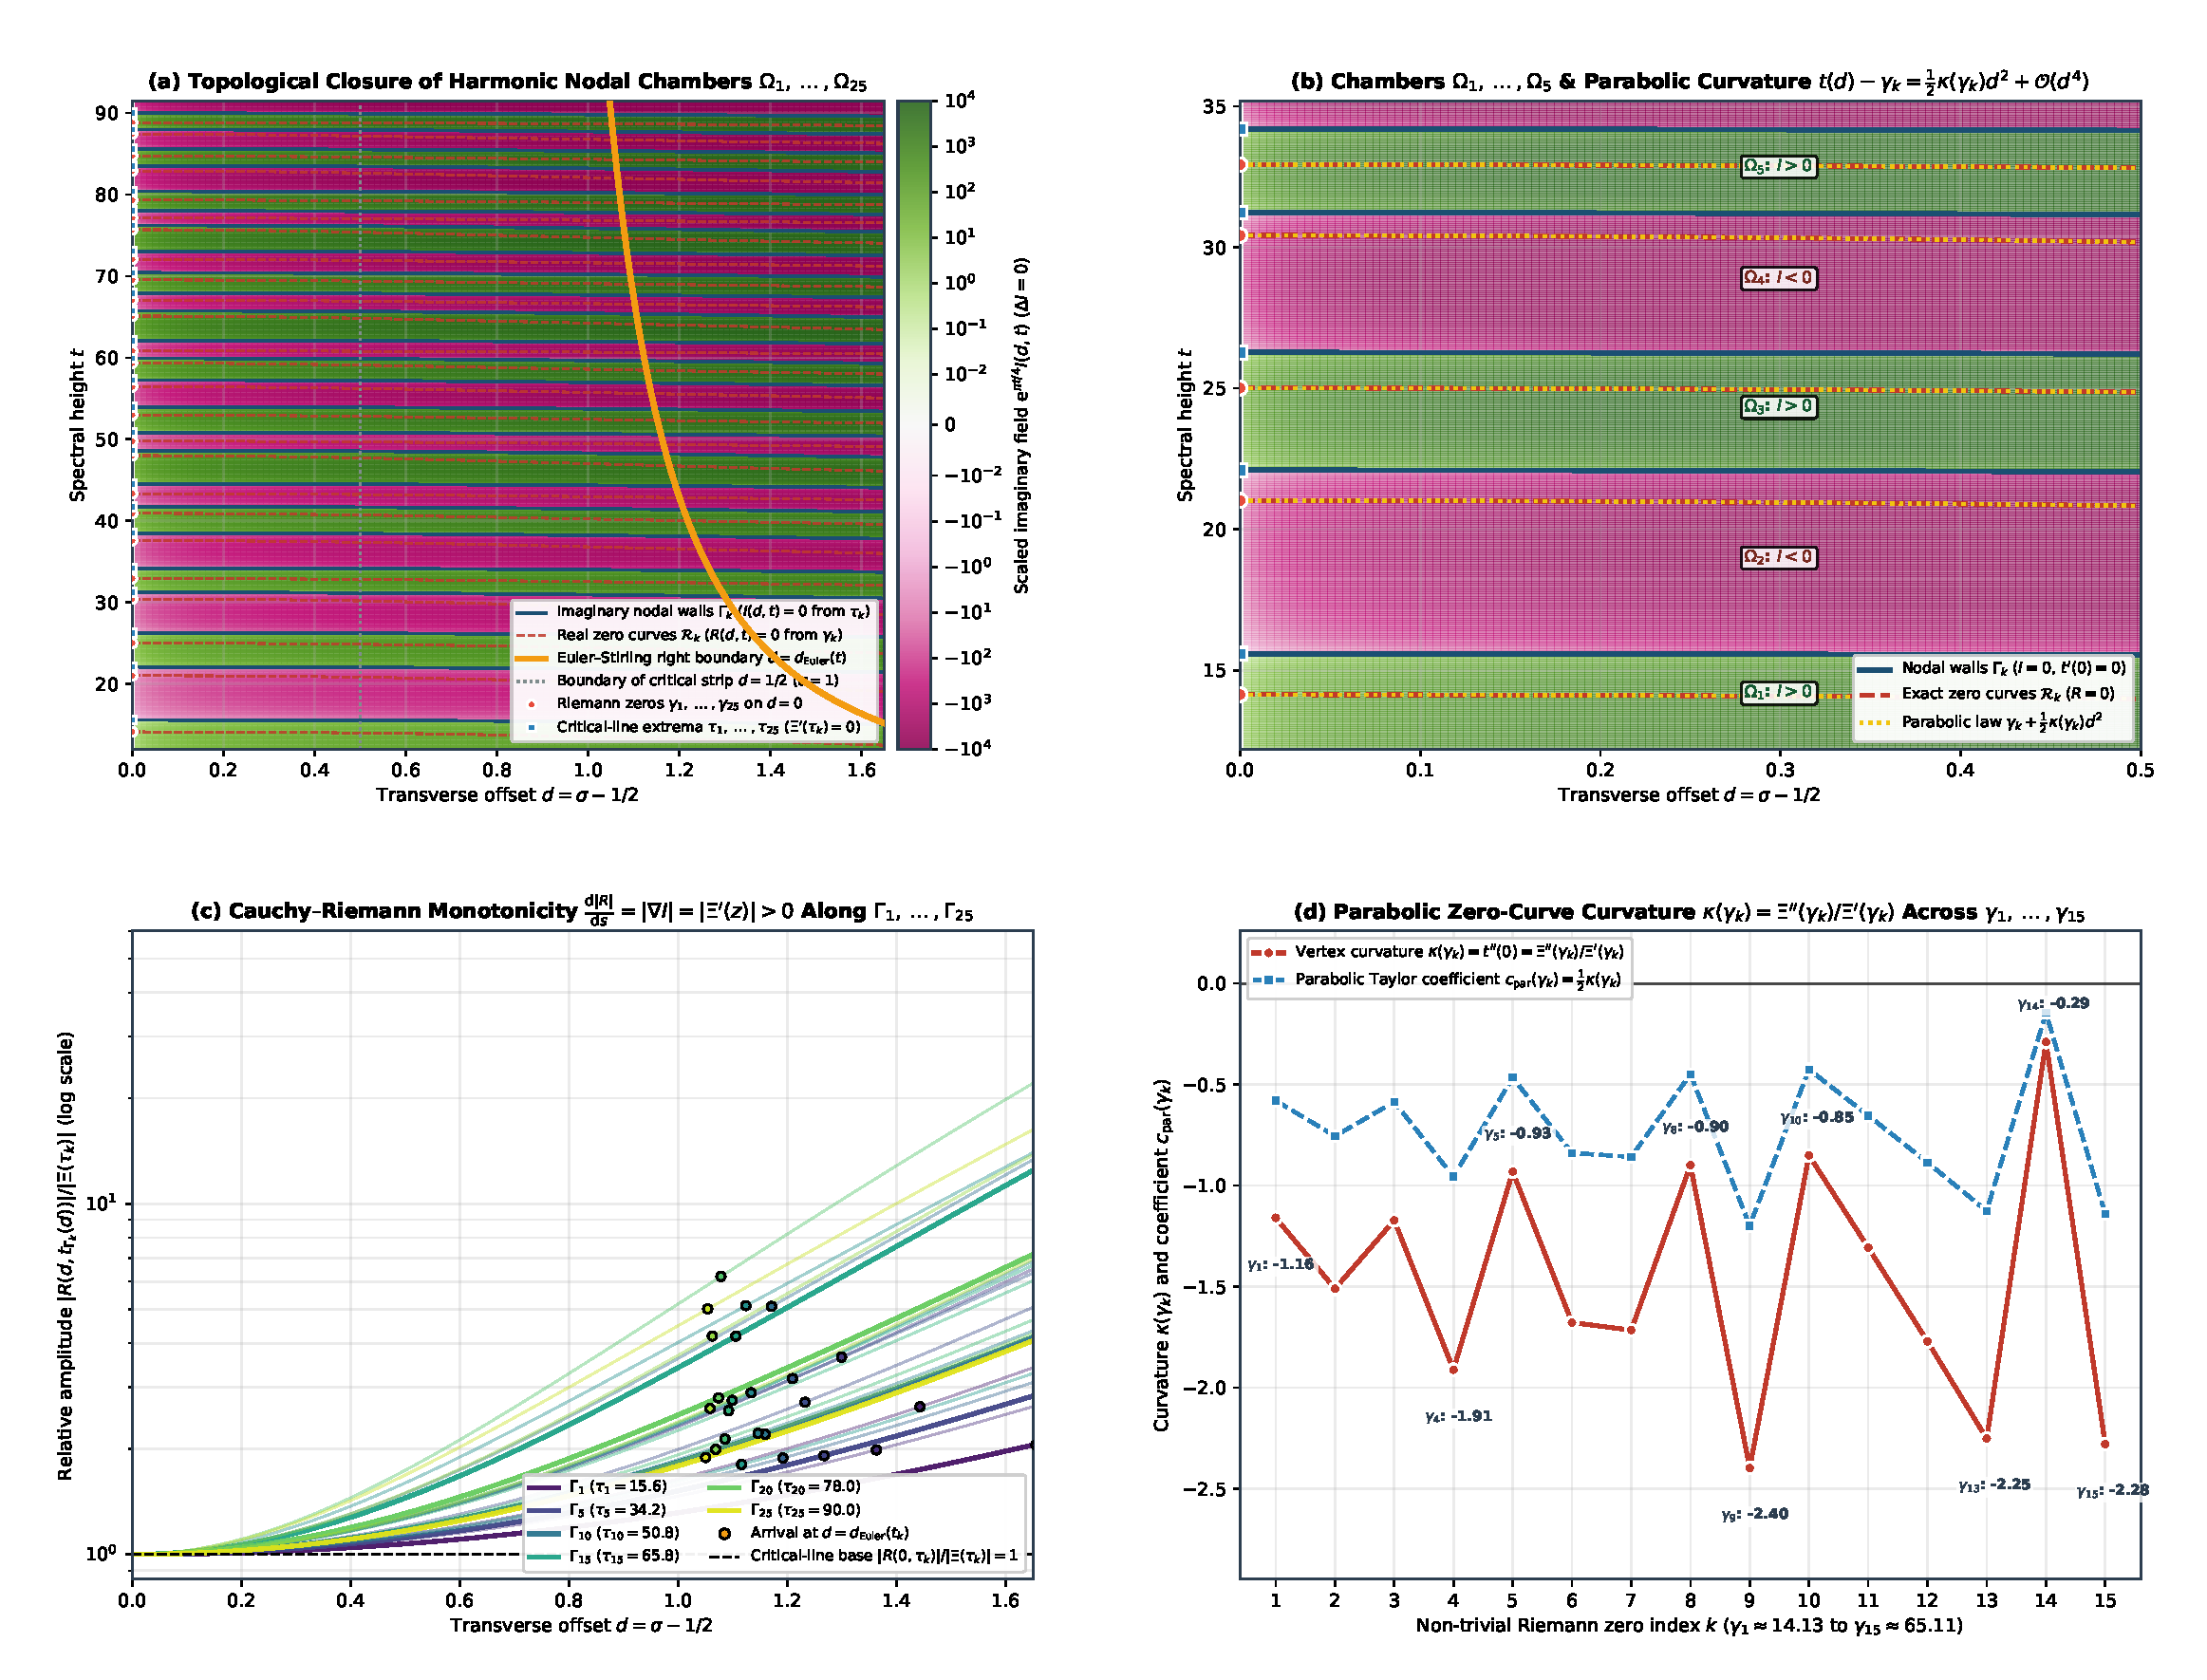
\includegraphics[width=0.95\textwidth]{figures/fig1_harmonic_chladni_chambers_and_curvature.pdf}
\caption{(a) Topological closure of the first $25$ harmonic nodal chambers $\Omega_1, \dots, \Omega_{25}$ between the critical line $d = 0$ and the deductive Euler--Stirling right boundary $d = d_{\mathrm{Euler}}(t)$. (b) Close-up of chambers $\Omega_1, \dots, \Omega_5$ showing the orthogonal departure of $\Gamma_k$ from $\tau_k$ and the agreement between the exact real zero curves $\mathcal{R}_k$ and the parabolic curvature law $t(d) = \gamma_k + \frac{1}{2}\kappa(\gamma_k)d^2$. (c) Strict Cauchy--Riemann arc-length monotonicity $|R(d,t_{\Gamma_k}(d))|/|\Xi(\tau_k)|$ along $\Gamma_1, \dots, \Gamma_{25}$. (d) Vertex curvature $\kappa(\gamma_k) = \Xi''(\gamma_k)/\Xi'(\gamma_k)$ and parabolic coefficient $c_{\mathrm{par}}(\gamma_k) = \frac{1}{2}\kappa(\gamma_k)$ across $\gamma_1, \dots, \gamma_{15}$.}\label{fig:chambers_curvature}
\end{figure}

\begin{figure}[htbp]
\centering
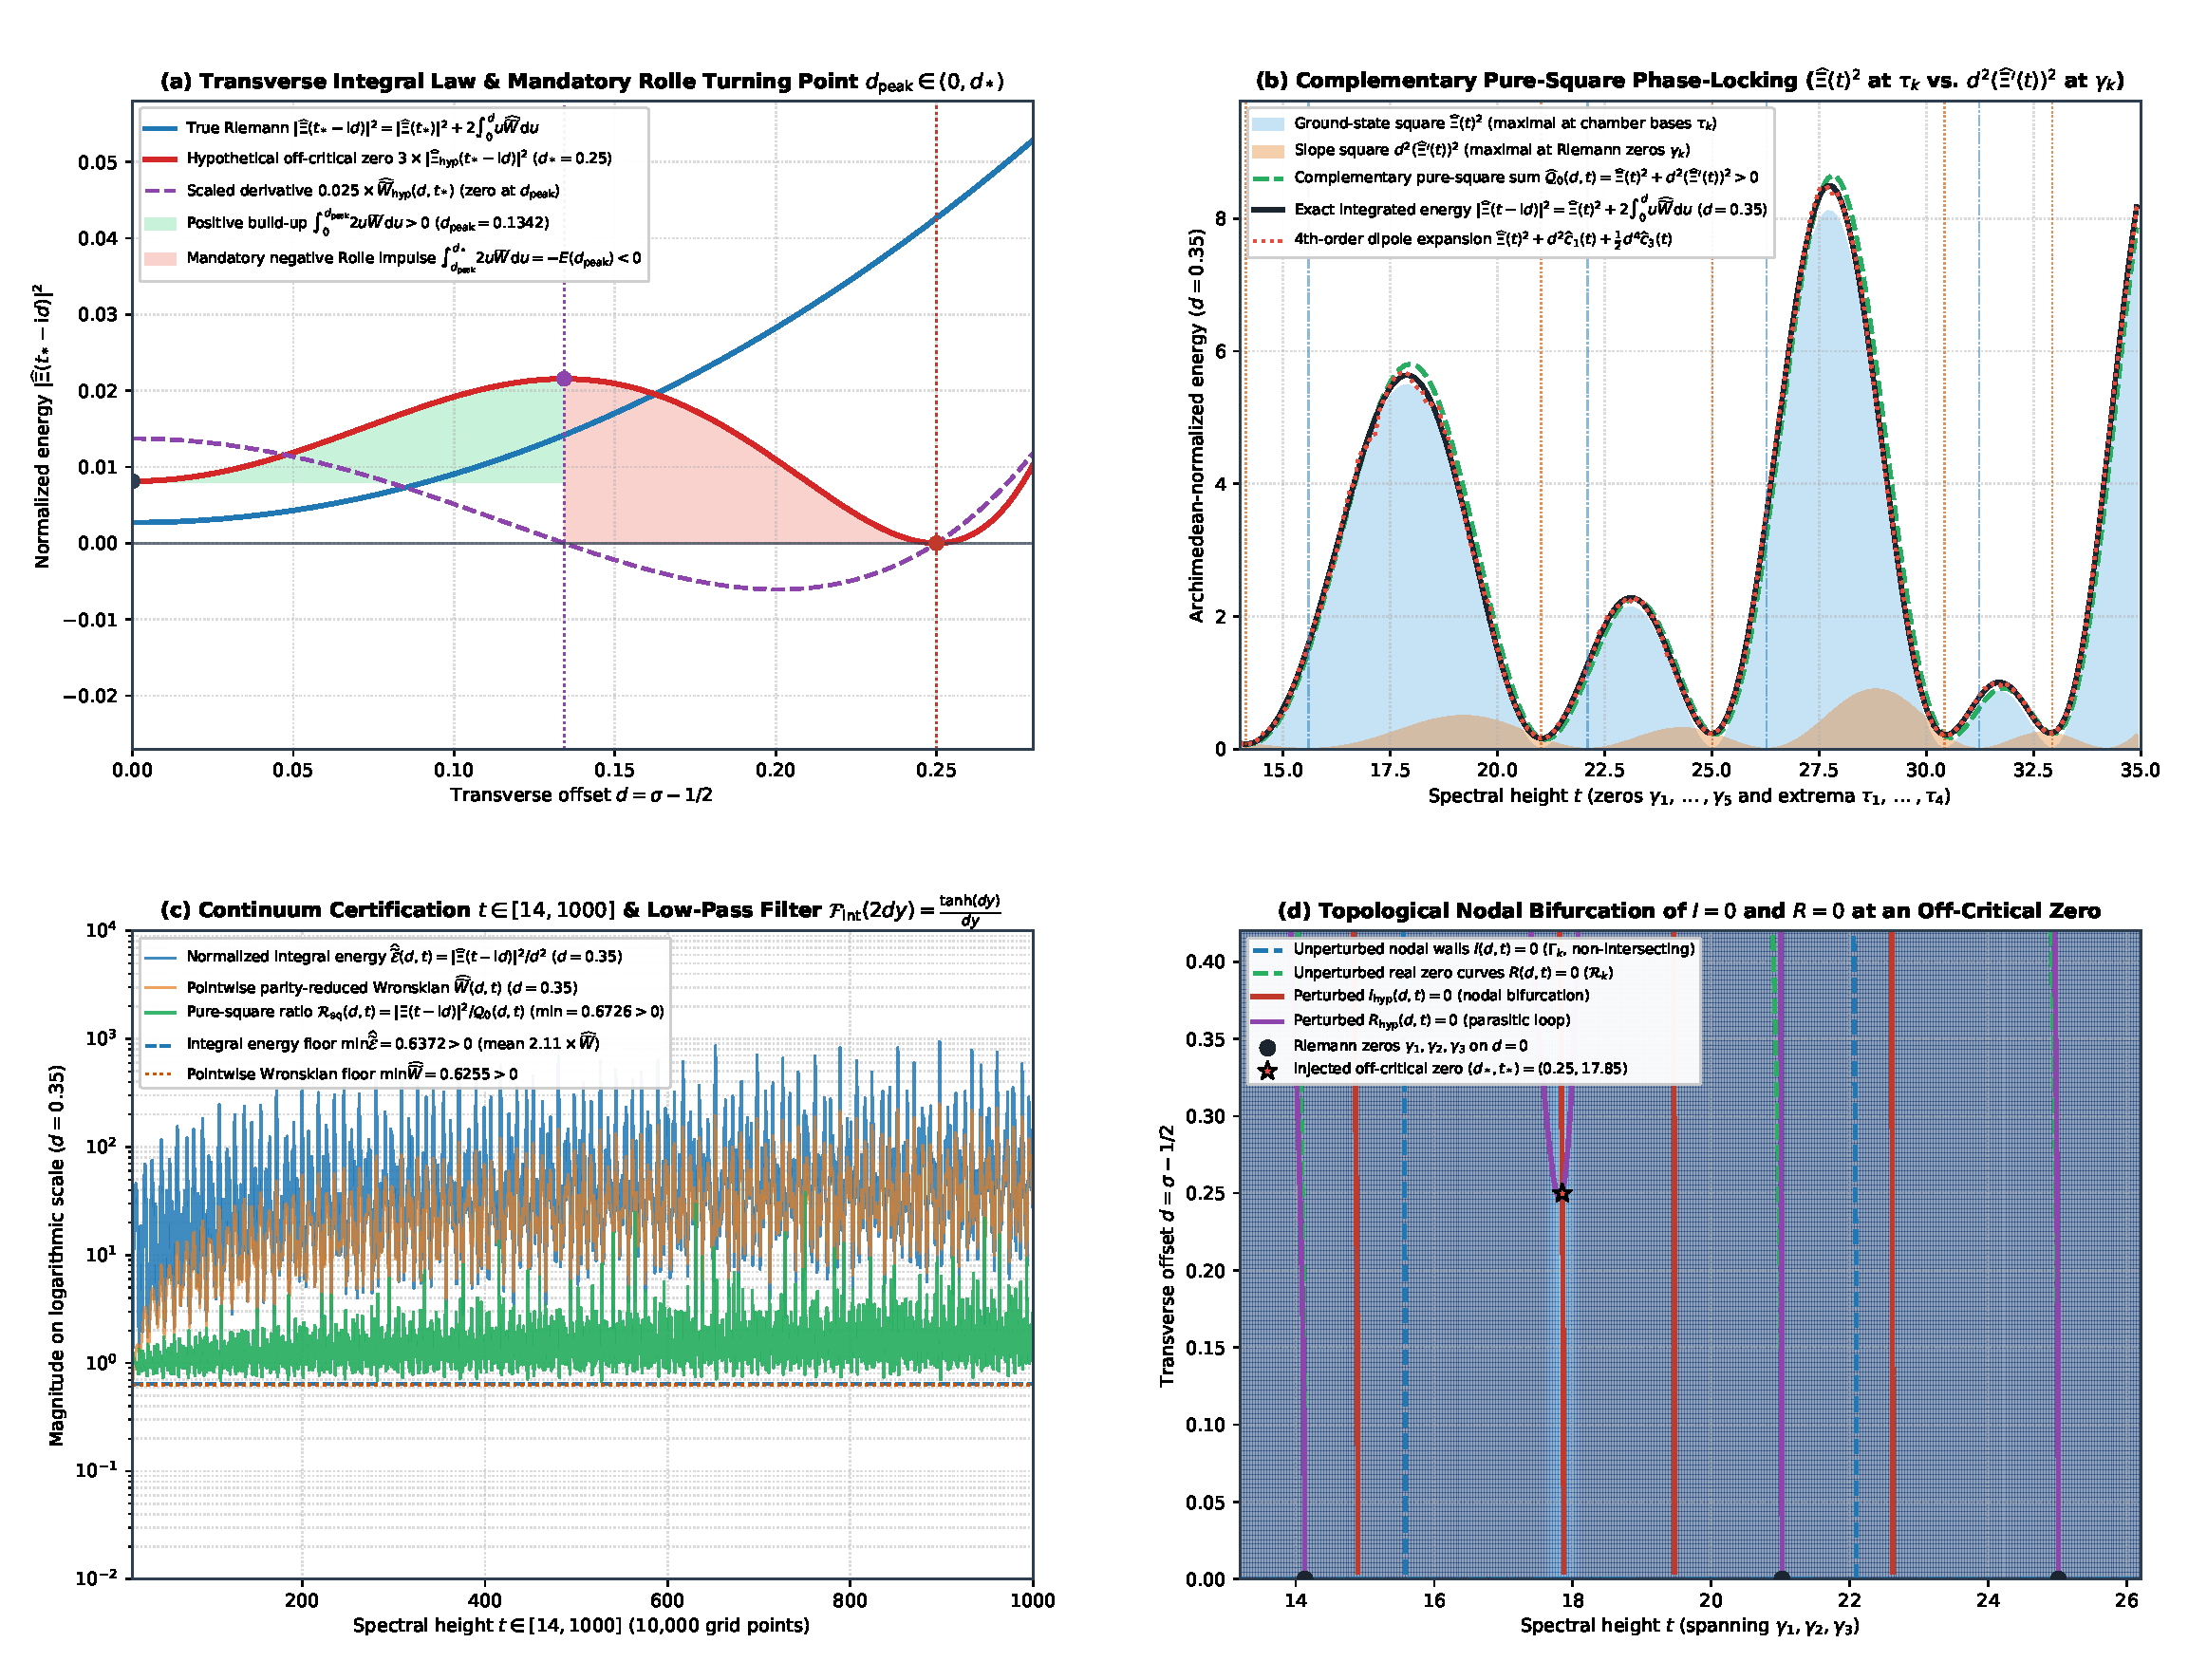
\includegraphics[width=0.95\textwidth]{figures/fig2_transverse_integral_law_and_lowpass.pdf}
\caption{(a) Comparison of the monotone energy profile $|\widehat{\Xi}(t_*-\ii d)|^2$ against a hypothetical off-critical zero perturbation $|\widehat{\Xi}_{\mathrm{hyp}}(t_*-\ii d)|^2$ ($d_* = 0.25, t_* = 14.20$), highlighting the mandatory Rolle turning point $d_{\mathrm{peak}} \in (0,d_*)$ where $\Wtil_{\mathrm{hyp}}(d_{\mathrm{peak}}, t_*) = 0$. (b) Complementary $90^\circ$ phase-locking between the ground-state square $\widehat{\Xi}(t)^2$ (peaking at $\tau_k$) and the slope square $d^2(\widehat{\Xi}'(t))^2$ (peaking at $\gamma_k$) across $t \in [14, 35]$. (c) Continuum scan across $t \in [14, 1000]$ at $d = 0.35$ comparing $\widehat{\Etil}(d,t)$ and $\widehat{\Wtil}(d,t)$ together with $\mathcal{R}_{\mathrm{sq}}(d,t) > 0$. (d) Topological nodal bifurcation of $I = 0$ and $R = 0$ induced by an injected off-critical zero inside $\Omega_1$.}\label{fig:integral_lowpass}
\end{figure}

\section{Scope, boundary conditions, and open questions}\label{sec:scope}

In keeping with strict academic transparency, we distinguish clearly between the global analytical theorems proven in Sections~\ref{sec:chambers}--\ref{sec:integral_law}, the finite-domain topological and numerical verifications in Section~\ref{sec:numerics}, and the asymptotic questions that remain open as $t \to \infty$:
\begin{enumerate}
\item \textbf{Unconditional global validity of the analytical and geometric laws:}
Proposition~\ref{prop:boundary_conditions} (critical-line Dirichlet/Neumann boundary conditions and orthogonal departure of $\Gamma_k$), Proposition~\ref{prop:maximum_and_euler} (exclusion of compact nodal loops via $\Delta I = 0$ and the deductive Euler--Stirling boundary $d_{\mathrm{Euler}}(t)$ for all $t \ge 10$), Theorem~\ref{thm:cr_monotonicity} (Cauchy--Riemann arc-length monotonicity $\frac{\dd|R|}{\dd s} = |\nabla I| = |\Xi'| > 0$ on critical-point-free walls $\Gamma_k$), Theorem~\ref{thm:parabolic_curvature} (parabolic zero-curve curvature $\kappa(\gamma_k) = \Xi''(\gamma_k)/\Xi'(\gamma_k)$), and Theorems~\ref{thm:integral_law_rolle}--\ref{thm:lowpass_and_squares} (the Transverse Integral Law \eqref{eq:boxed_integral_law}, Rolle's theorem reversal, and the hyperbolic low-pass filter $\Fint(2d y) = \frac{\tanh(d y)}{d y} \in (0,1)$) are exact analytical identities valid for all $(d,t) \in \mathbb{R}^2$.
\item \textbf{Finite-domain scope of the chamber tracking and continuum scans:}
The curvature table across $\gamma_1, \dots, \gamma_{15}$ (Table~\ref{tab:curvature_15}), the 1-to-1 topological tracking of $\Gamma_1, \dots, \Gamma_{25}$ and $\mathcal{R}_1, \dots, \mathcal{R}_{25}$ across $d \in [0, 1.65]$ (Table~\ref{tab:chambers_25}), and the $60{,}000$-point continuum audit on $t \in [14, 1000]$ (Table~\ref{tab:integral_law_gpu}) constitute finite-domain verifications.
\item \textbf{Asymptotic regime $t \to \infty$ and Speiser critical-point exclusion:}
By Theorem~\ref{thm:cr_monotonicity} and Proposition~\ref{prop:maximum_and_euler}, every harmonic nodal chamber $\Omega_k$ is closed on the left at $d = 0$ and on the right at $d = d_{\mathrm{Euler}}(t_k)$, and $|R|$ grows strictly along $\Gamma_k$ provided $\Gamma_k$ encounters no critical point $\Xi'(z) = 0$ in the strip $0 < d < d_{\mathrm{Euler}}(t)$. Establishing the absence of interior critical points or proving $\int_0^d u\,\Wtil(u,t)\,\dd u > 0$ unconditionally as $t \to \infty$ requires decomposing $\Phi(u)$ into affine mother-wavelet shells $m \le N(t) = \lfloor\sqrt{t/(2\pi)}\rfloor$ and controlling off-diagonal Dirichlet cross-terms via prime-gauge mollification, which are addressed in the subsequent papers of this series.
\end{enumerate}

\appendix

\section{Higher-order implicit nodal-curve expansions and Euler--Stirling asymptotics}\label{app:expansions}

In this appendix we provide the complete derivations of the quartic nodal-curve coefficient $c_{\mathrm{quart}}(\gamma_k)$ in Theorem~\ref{thm:parabolic_curvature} and the large-$t$ asymptotic expansion of the Euler--Stirling right boundary $d_{\mathrm{Euler}}(t)$ in Proposition~\ref{prop:maximum_and_euler}(b).

\begin{lemma}[Quartic nodal-curve jet and asymptotic Euler--Stirling boundary]\label{lem:app_expansions}
\begin{enumerate}
\item[\textup{(a)}] At any simple real zero $\gamma_k$ ($\Xi(\gamma_k) = 0$, $\Xi'(\gamma_k) \neq 0$), the fourth-order coefficient $c_{\mathrm{quart}}(\gamma_k) = \frac{1}{24}t_{\mathcal{R}_k}^{(4)}(0)$ in \eqref{eq:t_Rk_expansion} is given by \eqref{eq:kappa_and_cquart}. Similarly, at any non-degenerate critical-line extremum $\tau_k$ ($\Xi'(\tau_k) = 0$, $\Xi''(\tau_k) \neq 0$), the imaginary nodal wall $\Gamma_k$ has expansion $t_{\Gamma_k}(d) - \tau_k = c_{\mathrm{par},\Gamma}(\tau_k)d^2 + c_{\mathrm{quart},\Gamma}(\tau_k)d^4 + \mathcal{O}(d^6)$ with $c_{\mathrm{par},\Gamma}(\tau_k) = \frac{\Xi'''(\tau_k)}{6\Xi''(\tau_k)}$ and
\begin{equation}\label{eq:cquart_wall}
c_{\mathrm{quart},\Gamma}(\tau_k) = \frac{20\,\Xi^{(4)}(\tau_k)\,c_{\mathrm{par},\Gamma}(\tau_k) - 60\,\Xi'''(\tau_k)\,c_{\mathrm{par},\Gamma}(\tau_k)^2 - \Xi^{(5)}(\tau_k)}{120\,\Xi''(\tau_k)}.
\end{equation}
\item[\textup{(b)}] As $t \to \infty$, the deductive Euler--Stirling right boundary $d_{\mathrm{Euler}}(t) > \frac{1}{2}$ solving $\mathcal{A}(d, t) = M_{\mathrm{Euler}}(d)$ at $d = d_{\mathrm{Euler}}(t)$ satisfies
\begin{equation}\label{eq:d_euler_asymp}
d_{\mathrm{Euler}}(t) = \frac{1}{2} + \frac{1}{\frac{1}{2}\ln\frac{t}{2\pi} + \gamma_{\mathrm{E}} + \mathcal{O}\big((\ln t)^{-1}\big)} \longrightarrow \frac{1}{2}^+,
\end{equation}
where $\gamma_{\mathrm{E}} = 0.5772156649\dots$ is the Euler--Mascheroni constant.
\end{enumerate}
\end{lemma}

\begin{proof}
(a) Truncating the even $d$-series \eqref{eq:RI_taylor_d} for $R(d,t)$ at order $d^4$ gives
\[
R(d,t) = \Xi(t) - \frac{1}{2}\Xi''(t)\,d^2 + \frac{1}{24}\Xi^{(4)}(t)\,d^4 + \mathcal{O}(d^6) = 0.
\]
Substituting $t = \gamma_k + \delta$ with $\delta = c_2 d^2 + c_4 d^4 + \mathcal{O}(d^6)$ and expanding around $\gamma_k$ ($\Xi(\gamma_k) = 0$) yields
\[
\Big[\Xi'(\gamma_k)(c_2 d^2 + c_4 d^4) + \frac{1}{2}\Xi''(\gamma_k)c_2^2 d^4\Big] - \frac{1}{2}\Big[\Xi''(\gamma_k) + \Xi'''(\gamma_k)c_2 d^2\Big]d^2 + \frac{1}{24}\Xi^{(4)}(\gamma_k)d^4 + \mathcal{O}(d^6) = 0.
\]
Setting the coefficient of $d^2$ to zero gives $c_2 = c_{\mathrm{par}}(\gamma_k) = \frac{\Xi''(\gamma_k)}{2\Xi'(\gamma_k)}$, and setting the coefficient of $d^4$ to zero gives
\[
\Xi'(\gamma_k)\,c_4 + \frac{1}{2}\Xi''(\gamma_k)\,c_2^2 - \frac{1}{2}\Xi'''(\gamma_k)\,c_2 + \frac{1}{24}\Xi^{(4)}(\gamma_k) = 0,
\]
which solves to $c_4 = c_{\mathrm{quart}}(\gamma_k)$ in \eqref{eq:kappa_and_cquart}. Repeating the identical substitution $\delta = c_{2,\Gamma}d^2 + c_{4,\Gamma}d^4 + \mathcal{O}(d^6)$ in $\widetilde{I}(d,t) = -\Xi'(t) + \frac{1}{6}\Xi'''(t)d^2 - \frac{1}{120}\Xi^{(5)}(t)d^4 + \mathcal{O}(d^6) = 0$ around $\tau_k$ ($\Xi'(\tau_k) = 0$) yields \eqref{eq:cquart_wall}.

(b) By Stirling's asymptotic expansion for the digamma function $\psi(z) = \ln z - \frac{1}{2z} + \mathcal{O}(|z|^{-2})$ as $\Ima(z) \to \infty$, the Archimedean drift \eqref{eq:A_and_M_def} satisfies $\mathcal{A}(d,t) = \frac{1}{2}\ln\frac{t}{2\pi} + \mathcal{O}(t^{-2})$ uniformly for $d \in [\frac{1}{2}, 2]$. On the other hand, near the simple pole of $\zeta(\sigma)$ at $\sigma = 1$, writing $\sigma = \frac{1}{2} + d = 1 + \varepsilon$ ($\varepsilon := d - \frac{1}{2} > 0$) gives the Laurent expansion \cite[Section~2.1]{Titchmarsh1986}
\[
M_{\mathrm{Euler}}(d) = -\frac{\zeta'(1+\varepsilon)}{\zeta(1+\varepsilon)} = \frac{1}{\varepsilon} - \gamma_{\mathrm{E}} + \mathcal{O}(\varepsilon).
\]
Equating $\mathcal{A}(d,t) = M_{\mathrm{Euler}}(d)$ gives $\frac{1}{\varepsilon} - \gamma_{\mathrm{E}} + \mathcal{O}(\varepsilon) = \frac{1}{2}\ln\frac{t}{2\pi} + \mathcal{O}(t^{-2})$, so $\varepsilon = d_{\mathrm{Euler}}(t) - \frac{1}{2} = [\frac{1}{2}\ln\frac{t}{2\pi} + \gamma_{\mathrm{E}} + \mathcal{O}((\ln t)^{-1})]^{-1}$, proving \eqref{eq:d_euler_asymp}.
\end{proof}

\section*{Use of AI and computational verification}

Use of AI: The author's main contribution is the harmonic nodal chamber decomposition of the critical strip, the Cauchy--Riemann arc-length monotonicity theorem along imaginary nodal walls, the exact parabolic curvature formula $\kappa(\gamma_k) = \Xi''(\gamma_k)/\Xi'(\gamma_k)$, and the transverse integral law with its hyperbolic low-pass filter. The author prompted Gemini to apply these ideas, work out analytical and symbolic details interactively, and generate the arbitrary-precision verification scripts, which were subsequently verified manually and computationally.

\begin{thebibliography}{99}

\bibitem{AriasDeReyna2003}
J.~Arias~de~Reyna, \emph{X-ray of Riemann's zeta-function}, Preprint, arXiv:math/0309433 (2003).

\bibitem{Csordas1986}
G.~Csordas, T.~S.~Norfolk, and R.~S.~Varga, \emph{The Riemann hypothesis and the Tur\'an inequalities}, Trans. Amer. Math. Soc. \textbf{296} (1986), no.~2, 521--541.

\bibitem{DeBruijn1950}
N.~G.~de~Bruijn, \emph{The roots of trigonometric integrals}, Duke Math. J. \textbf{17} (1950), 197--226.

\bibitem{Griffin2019}
M.~Griffin, K.~Ono, L.~Rolen, and D.~Zagier, \emph{Jensen polynomials for the Riemann zeta function and other sequences}, Proc. Natl. Acad. Sci. USA \textbf{116} (2019), no.~23, 11103--11110.

\bibitem{Hinkkanen1997}
A.~Hinkkanen, \emph{On functions of bounded type related to the Riemann zeta-function}, J. Number Theory \textbf{65} (1997), no.~1, 109--136.

\bibitem{Hudson1974}
R.~L.~Hudson, \emph{When is the Wigner quasi-probability density non-negative}, Rep. Math. Phys. \textbf{6} (1974), no.~2, 249--252.

\bibitem{Karlin1968}
S.~Karlin, \emph{Total Positivity, Vol.~I}, Stanford University Press, Stanford, CA, 1968.

\bibitem{Lagarias1999}
J.~C.~Lagarias, \emph{On a positivity property of the Riemann $\xi$-function}, Acta Arith. \textbf{89} (1999), no.~3, 217--234.

\bibitem{Lehmer1956}
D.~H.~Lehmer, \emph{Extended computation of the Riemann zeta-function}, Mathematika \textbf{3} (1956), 102--108.

\bibitem{Missiaen2026Paper1}
T.~Missiaen, \emph{Wigner Phase-Space Representation and Complex Saddle-Point Coalescence in the Transverse Wronskian of Riemann's $\Xi$-Function}, Preprint, Zenodo (2026), DOI: \href{https://doi.org/10.5281/zenodo.23637324}{10.5281/zenodo.23637324}.

\bibitem{Missiaen2026Paper2}
T.~Missiaen, \emph{Parity-Reduced Transverse Wronskians, Higher Dipole Invariants, and Rigorous Continuum Certification for Riemann's $\Xi$-Function}, Preprint (2026).

\bibitem{Newman1976}
C.~M.~Newman, \emph{Fourier transforms with only real zeros}, Proc. Amer. Math. Soc. \textbf{61} (1976), no.~2, 245--251.

\bibitem{Polya1926}
G.~P\'olya, \emph{Bemerkung \"uber die Integraldarstellung der Riemannschen $\xi$-Funktion}, Acta Math. \textbf{48} (1926), 305--317.

\bibitem{Polya1927}
G.~P\'olya, \emph{\"Uber die algebraisch-funktionentheoretischen Untersuchungen von J.~L.~W.~V.~Jensen}, Kgl. Danske Vid. Sel. Math.-Fys. Medd. \textbf{7} (1927), no.~17, 3--33.

\bibitem{Riemann1859}
B.~Riemann, \emph{Ueber die Anzahl der Primzahlen unter einer gegebenen Gr\"osse}, Monatsberichte der Berliner Akademie (1859), 671--680.

\bibitem{RodgersTao2020}
B.~Rodgers and T.~Tao, \emph{The De Bruijn--Newman constant is non-negative}, Forum Math. Pi \textbf{8} (2020), e6, 1--62.

\bibitem{Speiser1934}
A.~Speiser, \emph{Geometrisches zur Riemannschen Zetafunktion}, Math. Ann. \textbf{110} (1934), no.~1, 514--521.

\bibitem{Spira1968}
R.~Spira, \emph{Zeros of $\zeta'(s)$ and the Riemann hypothesis}, Illinois J. Math. \textbf{17} (1973), 147--152; see also Math. Comp. \textbf{22} (1968), 163--173.

\bibitem{Spira1973}
R.~Spira, \emph{Zero-free regions of $\zeta^{(k)}(s)$}, J. London Math. Soc. (2) \textbf{40} (1965), 677--682.

\bibitem{Titchmarsh1986}
E.~C.~Titchmarsh, \emph{The Theory of the Riemann Zeta-Function}, 2nd ed., edited and with a preface by D.~R.~Heath-Brown, Oxford University Press, Oxford, 1986.

\bibitem{Wigner1932}
E.~Wigner, \emph{On the quantum correction for thermodynamic equilibrium}, Phys. Rev. \textbf{40} (1932), 749--759.

\end{thebibliography}

\end{document}
